\documentclass{beamer}
% begin handouts 
%\documentclass[handout]{beamer}
%\usepackage{pgfpages}
%\pgfpagelayout{4 on 1}[a4paper,border shrink=5mm,landscape]
% end   handouts

\usepackage[utf8x]{inputenc} %Para poner acentos directamente
\usepackage{beamerthemesplit}
\usepackage{verbatim}
\usepackage{url}
 
%\usetheme{Bergen}
%\usetheme{Berlin} % se ven bien los nombres de autores
%\usetheme{Darmstadt}
\usetheme{Dresden} % se ven bien los nombres de autores
%\usetheme{Goettingen} %cosas raras, pero interesante igual
%\usetheme{Marburg} %cosas raras, pero interesante igual 
%\usetheme{Szeged}

\title{Buti\'a: Plataforma rob\'otica gen\'erica para la ense\~nanza de la inform\'atica}
\author[\Tiny{G. Tejera \and A. Aguirre \and F. Andrade \and P. Gindel \and S. Margni \and G. Reisch \and J. Visca}]{Gonzalo Tejera \and Andr\'es Aguirre \and \\~\\ Federico Andrade \and Pablo Gindel \and Santiago Margni \and Guillermo Reisch \and Jorge Visca}
\institute[InCo]{
\tiny{Instituto de Computación, Facultad de Ingeniería, Universidad de la República\\J. Herrera y Reissig 565, Montevideo, Uruguay\\
\href{http://www.fing.edu.uy/inco/proyectos/butia}{http://www.fing.edu.uy/inco/proyectos/butia} \\
\texttt{butia@fing.edu.uy}
}}

\date{4/03/2011}

\begin{document}

\frame{\titlepage}

\pgfdeclareimage[height=0.5cm]{congres-logo}{graphics/case2011.png}
\pgfdeclareimage[height=0.5cm]{butia-logo}{graphics/butia_logo.jpg}

\logo{\pgfuseimage{congres-logo}}

\setbeamertemplate{sidebar left}
{
\logo{\pgfuseimage{butia-logo}}
\vfill%
\rlap{\hskip0.1cm\insertlogo}%
\vskip9pt%
}
	
%\setbeamertemplate{navigation symbols}{} 
\setbeamertemplate{table of contents}{}

\section[Agenda]{}
\frame{\tableofcontents}


\setbeamertemplate{background canvas}{}

\section{Introducci\'on}
\subsection{Objetivos}
%FA
\begin{frame}
  \frametitle{Proyecto Buti\'a}
  \begin{center}
    \begin{itemize}
	    \item Crear una plataforma simple y econ\'omica que permita a alumnos de liceos p\'ublicos interiorizarse con la programaci\'on del comportamiento de robots
	    \item<2-> A trav\'es de la rob\'otica transmitir a profesores y estudiantes conocimientos b\'asicos sobre las nuevas tecnolog\'ias y sus aplicaciones
		\item<3-> Disminuir las asimetrías existentes entre liceos públicos y privados
		\item<4-> El proyecto fue financiado por la ANII y apoyado por la unidad de extensi\'on de la Facultad de Ingenier\'ia
	\end{itemize}
    \end{center}
\end{frame}


 \frame {
  \frametitle{Rob\'otica Educativa}
  \begin{center}
	\begin{itemize}
	    \item Programar los comportamientos de un robot m\'ovil genera mucho inter\'es en los adolescentes
	    \item<2-> Permite alcanzar resultados visuales inmediatos de sus programas
        \item<3-> Se estimula la creatividad
		\item<4-> Aprendizaje de conceptos b\'asicos de programaci\'on
        \item<5-> Uso de conocimientos adquiridos en otras disciplinas o asignaturas
	\end{itemize}
  \end{center}
}

\frame {
  \frametitle{Proyecto OLPC (One Laptop per Child)}
  \begin{center}
%	   \begin{right}
		   \begin{figure}
			 	 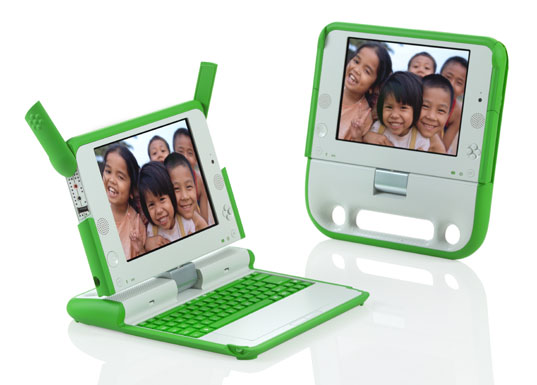
\includegraphics[scale=0.15]{graphics/xos.jpg}
		   \end{figure}
%	   \end{right}
	\begin{itemize}
	    \item El proyecto OLPC busca llevar una computadora con conectividad a cada ni\~no
	    \item<2-> Software: GNU/Linux y Sugar
        \item<3-> Hardware: Netbook de bajo consumo (computadora XO)
		\item<4-> En Uruguay es llevado a cabo por el plan Ceibal en primaria y secundaria
	\end{itemize}
  \end{center}
}

\frame {
  \frametitle{Transformando la XO en un robot m\'ovil}
  \begin{center}
	\begin{itemize}
	    \item XO es el \alert{``cerebro''} del robot
	    \item<2-> Interacci\'on con Hardware de la XO
		  \begin{itemize}
		 	   \item<2-> Webcam
			   \item<2-> Micr\'ofono
		  \end{itemize}
	    \item<3-> Interacci\'on con Software de la XO
		  \begin{itemize}
		 	   \item<3-> Tortugarte
			   \item<3-> Python
		  \end{itemize}
		\item<4-> Interacci\'on con sensores
		  \begin{itemize}
		 	   \item<4-> Luz, escala de grises, distancia, vibraci\'on, campo magn\'etico, inclinaci\'on, contacto, temperatura 
		  \end{itemize}
		\item<5-> Interacci\'on con actuadores
		  \begin{itemize}
		 	   \item<5-> Led, motores, pinza, display 
		  \end{itemize}
	\end{itemize}
  \end{center}
}

\section{Prototipo}
\subsection{Arquitectura Buti\'a}
%AA
\frame {
  \frametitle{Caracteristicas}
  \begin{itemize}
 	   \item<1-> Portable a plataformas con bajas prestaciones de hardware
	   \begin{itemize}
			\item<1-> Router dom\'estico Asus OpenWrt GNU/Linux (16MB RAM 8MB ROM)
			\item<1-> Computadora XO v1.0 (512MB RAM)
			\item<1-> Smart Phone
			\item<1-> Sistemas basados en Single Boards Computers (FoxBoard, BeagleBoard, HawkBoard)
	   \end{itemize}
 	   \item<2-> Enfoque modular
	   \item<3-> F\'acilmente extensible
	   \item<4-> Arquitectura orientada a capas
  \end{itemize}
}
\frame {
  \frametitle{Dise\~no}
   \begin{figure}
%			 Puertos para conectar sensores
	 	 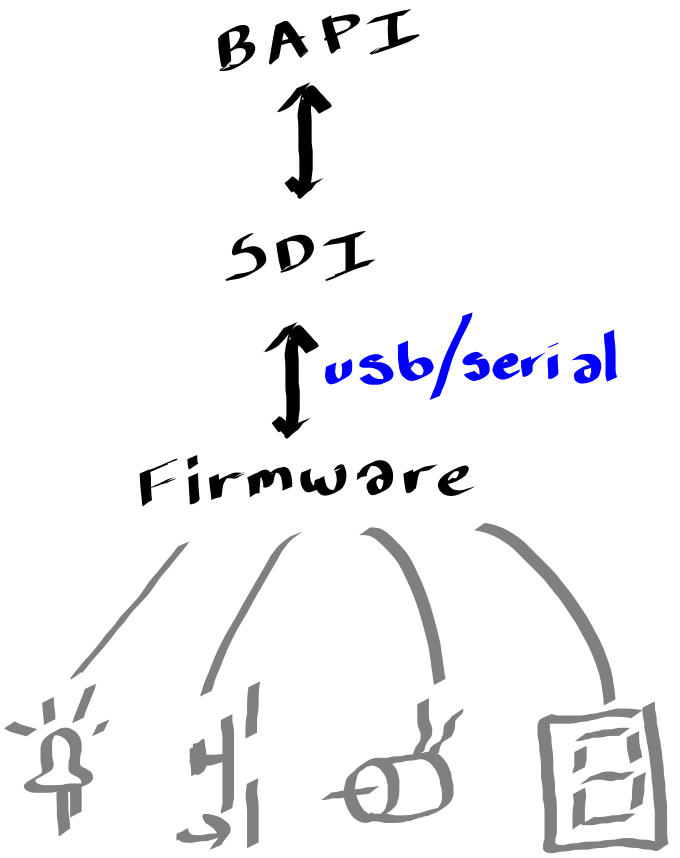
\includegraphics[scale=0.20]{graphics/diagrama_capas.png}
   \end{figure}
}
 
\frame {
  \frametitle{Capa Firmware}
  \begin{itemize}
 	   \item Encargada de la interaci\'on con el Hardware.
		  \begin{itemize}
		 	   \item Sensores y Actuadores
		  \end{itemize}
	   \item<2-> El hardware es abstra\'ido como \alert{m\'odulos} en la programaci\'on del firmware
		  \begin{itemize}	   			
				\item<2-> Motores, Luz, Grises, Distancia, ... 	
				\item<2-> Existe una Interfaz que cada m\'odulo debe cumplir
				\item<2-> Permite una f\'acil extensi\'on
		  \end{itemize}
	   \item<3-> Funcionalidades exportadas en servicios de software
	   \begin{itemize}				
			\item<3-> Motores:mover(sentido1, velocidad1, sentido2, velocidad2)
	   \end{itemize}
		\item<4-> Implementada en el Firmware del microcontrolador utilizado (PIC/ATMEL AVR)
  \end{itemize}
}
\frame {
  \frametitle{Capa Firmware - Plug \& Play}
%   \begin{center}
	   \begin{figure}
%			 Puertos para conectar sensores
		 	 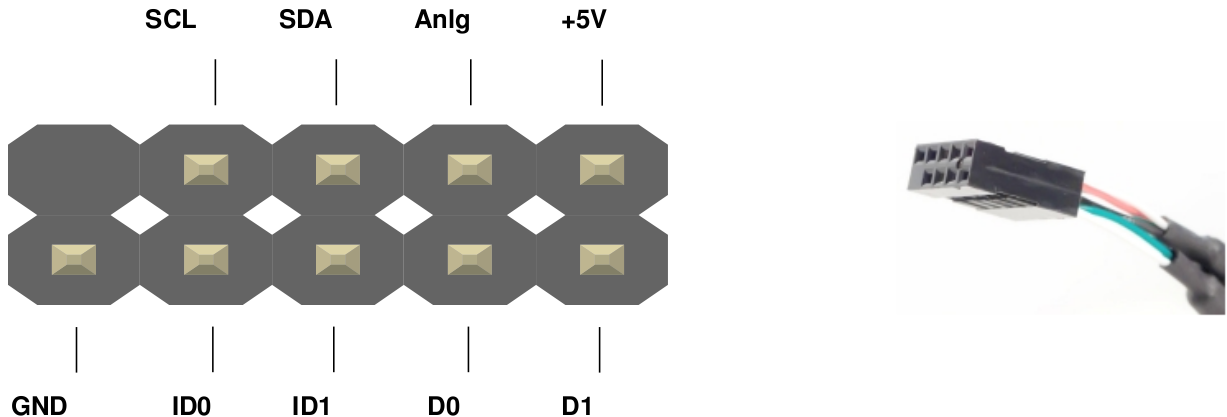
\includegraphics[scale=0.20]{graphics/conector_butia.png}
	   \end{figure}
%   \end{center}  
  \begin{itemize}
 	   \item<1-> Cada conector posee pines de identificaci\'on
	   \item<2-> El firmware identifica al sensor y le asigna un m\'odulo	
	   \item<3-> La lista de m\'odulos presentes en el hardware es notificada a la capa superior
  \end{itemize}
}
\frame {
  \frametitle{Capa 2 - Service Discovery and Invocation}
  \begin{itemize}
	 \item Descubrimiento din\'amico de m\'odulos
	 \item<2-> Descubrimiento din\'amico de servicios
	 \item<3-> Invocaci\'on de servicios
     %\item<1-> Extender los servicios a trav\'es de drivers
     %\item<1-> Exporner servicios digeridos hacia aplicaci\'on
	 \item<4-> Brinda independencia de la placa de entrada/salida
		   \begin{itemize}
				\item<4-> Arduino
				\item<4-> USB4all
				\item<4-> GoGo board
		   \end{itemize}
	 \item<5-> Brinda independencia de la tecnolog\'ia de comunicaci\'on con la placa de entrada/salida
		   \begin{itemize}
				\item<5-> USB
				\item<5-> Serial
				\item<5-> Bluetooth
		   \end{itemize}
	 \item<6-> Puede ser ejecutada en una XO/PC/SBC
  \end{itemize}
}
\frame {
  \frametitle{Capa3 - Buti\'a Application Programming Interface}
  \begin{itemize}
 	  \item Brinda una interfaz de alto nivel para poder interactuar con los m\'odulos
	  \begin{itemize}
	    \item LIST
    	\item DESCRIBE moduleName
		\item CALL moduleName operation param1, param2, ... , paramN
	  \end{itemize}
	  \item<2-> Los clientes se implementan sobre esta capa utilizando dichas primitivas
	  \begin{itemize}
	  	\item<2-> Existe un cliente (bobot-server) que expone este protocolo en la red
	  \end{itemize}
  \end{itemize}
}

\frame {
  \frametitle{Ventajas y Desventajas}
  \begin{itemize}
    \item Ventajas
	\begin{itemize}
	   \item<2-> F\'acil extensi\'on
 	   \begin{itemize}
	   \item<2-> No es necesario preocuparse por aspectos relacionados con la comunicaci\'on o detalles de bajo nivel del firmware
	   \item<2-> Solo hay que centrarse en la l\'ogica de control del sensor/actuador a controlar
	   \end{itemize}
 	   \item<3-> Mantenible
	   \begin{itemize}
	   \item<3-> Comportamiento del robot implementado en lenguaje de alto nivel, en firmware, solo la l\'ogica de control del sensor/actuador
	   \end{itemize}
	   \item<4-> Autoconfigurable
	   \begin{itemize}
			\item<4-> Plug \& Play y descubrimiento de m\'odulos y servicios elimina etapa de configuraci\'on
	   \end{itemize}
  	\end{itemize}
  \end{itemize}
}

\frame {
  \frametitle{Ventajas y Desventajas}
  \begin{itemize}
    \item Desventajas
	\begin{itemize}
	   \item Mayor overhead en procesamiento con poco imp\'acto en la performance
	   \item Mecanismo de Plug \& Play implementado utiliza muchos recursos de E/S
  	\end{itemize}
  \end{itemize}
}

\subsection{Implementaci\'on}
%AA

\frame {
  \frametitle{Componentes de Hardware}
 \begin{tabular}{cc}
   \hline
   Motores & Dynamixel AX12 \\
   \hline
   Control de bajo nivel & Arduino Mega \\
   \hline
   Control de alto nivel & Computadora OLPC \\
   \hline
   Chasis & Acr\'ilico 5mm \\
   \hline
   Amortiguaci\'on & Placa acero alto carbono 0.5mm \\
   \hline
   Sensores & Kit DFRobot para Arduino y sensores Sharp\\
   \hline

\end{tabular}

}
\frame {
  \frametitle{Componentes de Software}
  \begin{itemize}
	\item La Capa Firmware est\'a implementada C/C++ dependiendo de los lenguajes de programaci\'on soportados por el microcontrolador
	\item<2-> La Capa Service Discovery and Invocation y Buti\'a Application Programming Interface est\'an programados en Lua
	\begin{itemize}
		\item<2-> Lua es un lenguaje liviano y portable que lo hace muy adecuado para sistemas embebidos
	\end{itemize}	 
  \end{itemize}
}
\frame {
  \frametitle{Componentes de Software}
  \begin{itemize}
	\item Los clientes pueden escribirse en Lua o en otro lenguaje mediante una conexi\'on TCP/IP con bobot-server
	\item<2-> La comunicaci\'on con la placa de entrada/salida microcontrolada puede hacerse por USB o serial
	\begin{itemize}
		\item<2-> Microcontrolador PIC18f4550 utiliza USB, comunicaci\'on utilizando binding de libusb (lualibusb) para Lua desarrollado por el grupo
		\item<2-> Arduino utiliza conversor USB-serial, se utiliza biblioteca serialcomm implementada en C para comunicaci\'on serie 
	\end{itemize}
	 
  \end{itemize}
}

\subsection{Los niños toman el control}
\frame {
  \frametitle{Bloques Tortuga}
  \begin{itemize}
	   \item Lenguaje de programaci\'on ic\'onico denominado Bloques Tortuga (Turtle Blocks)
 	   \item<2-> Bloques Tortuga es una actividad gr\'afica de Sugar inspirada en el lenguaje de programaci\'on Logo
	   \item<3-> Permite construir programas "dibujando" con bloques
	   \item<4-> Estos bloques son elementos simples de programaci\'on visual
	   \item<5-> Pone a la altura de los ni\~nos los conceptos de programaci\'on 
  \end{itemize}
}
\frame {
  \frametitle{Paleta Butiá}
	   \begin{center}
		   \begin{figure}
		   		 Paleta Tortuga Buti\'a	
			 	 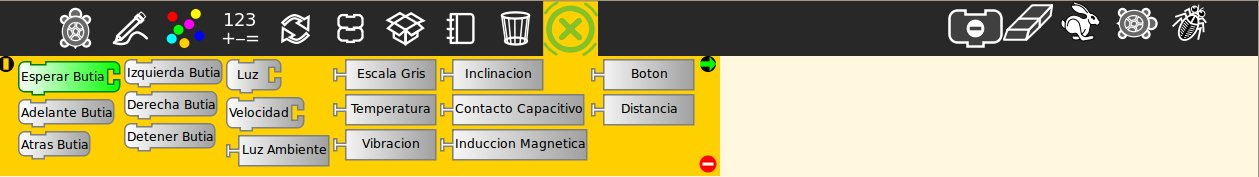
\includegraphics[scale=0.25]{graphics/paleta_butia.JPG}
		   \end{figure}
	   \end{center}
	   \begin{itemize}
	   		\item Paleta para controlar el robot
			\item<2-> Cada sensor es mostrado como un bloque
			\item<3-> Cada bloque puede ser probado individualmente
            %Es posible ejecutar un bloque haciendo click con el rat\'on sobre el mismo cuando est\'a ubicado en el \'area de programa.
	    \end{itemize}
}

\frame {
  \frametitle{Paleta Buti\'a}
	   \begin{center}
		   \begin{figure}
		   		 Paleta Tortuga Buti\'a	
			 	 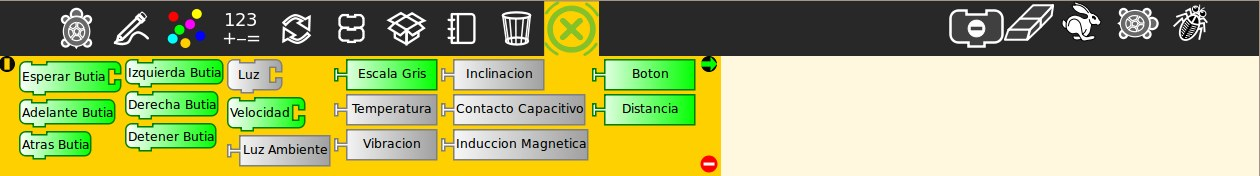
\includegraphics[scale=0.25]{graphics/paleta_butia_coloreada.JPG}
		   \end{figure}
	   \end{center}
	   \begin{itemize}
	       \item Plug \& Play: Se colorean los bloques de la paleta Buti\'a si el sensor correspondiente esta conectado
		   \item<2-> Desarrollo, depuraci\'on y ejecuci\'on sobre la misma plataforma
	    \end{itemize}
}

\frame {
  \frametitle{Programando Comportamientos}
  \begin{columns}
   \column[c]{6cm}
\begin{center}
  \begin{figure}
      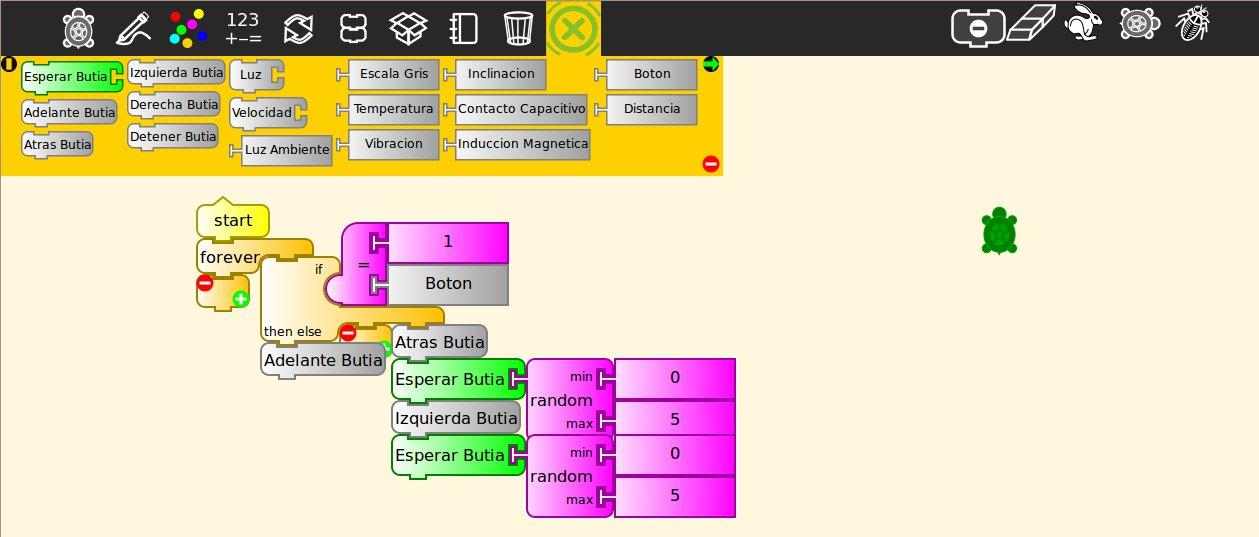
\includegraphics[scale=0.159]{graphics/tortuga_evitar_obstaculos.JPG}
  \end{figure}
  Programa para evitar obstaculos desarrollado en Tortuga
\end{center}
   \column[c]{4cm}
\begin{center}
  \begin{figure}
      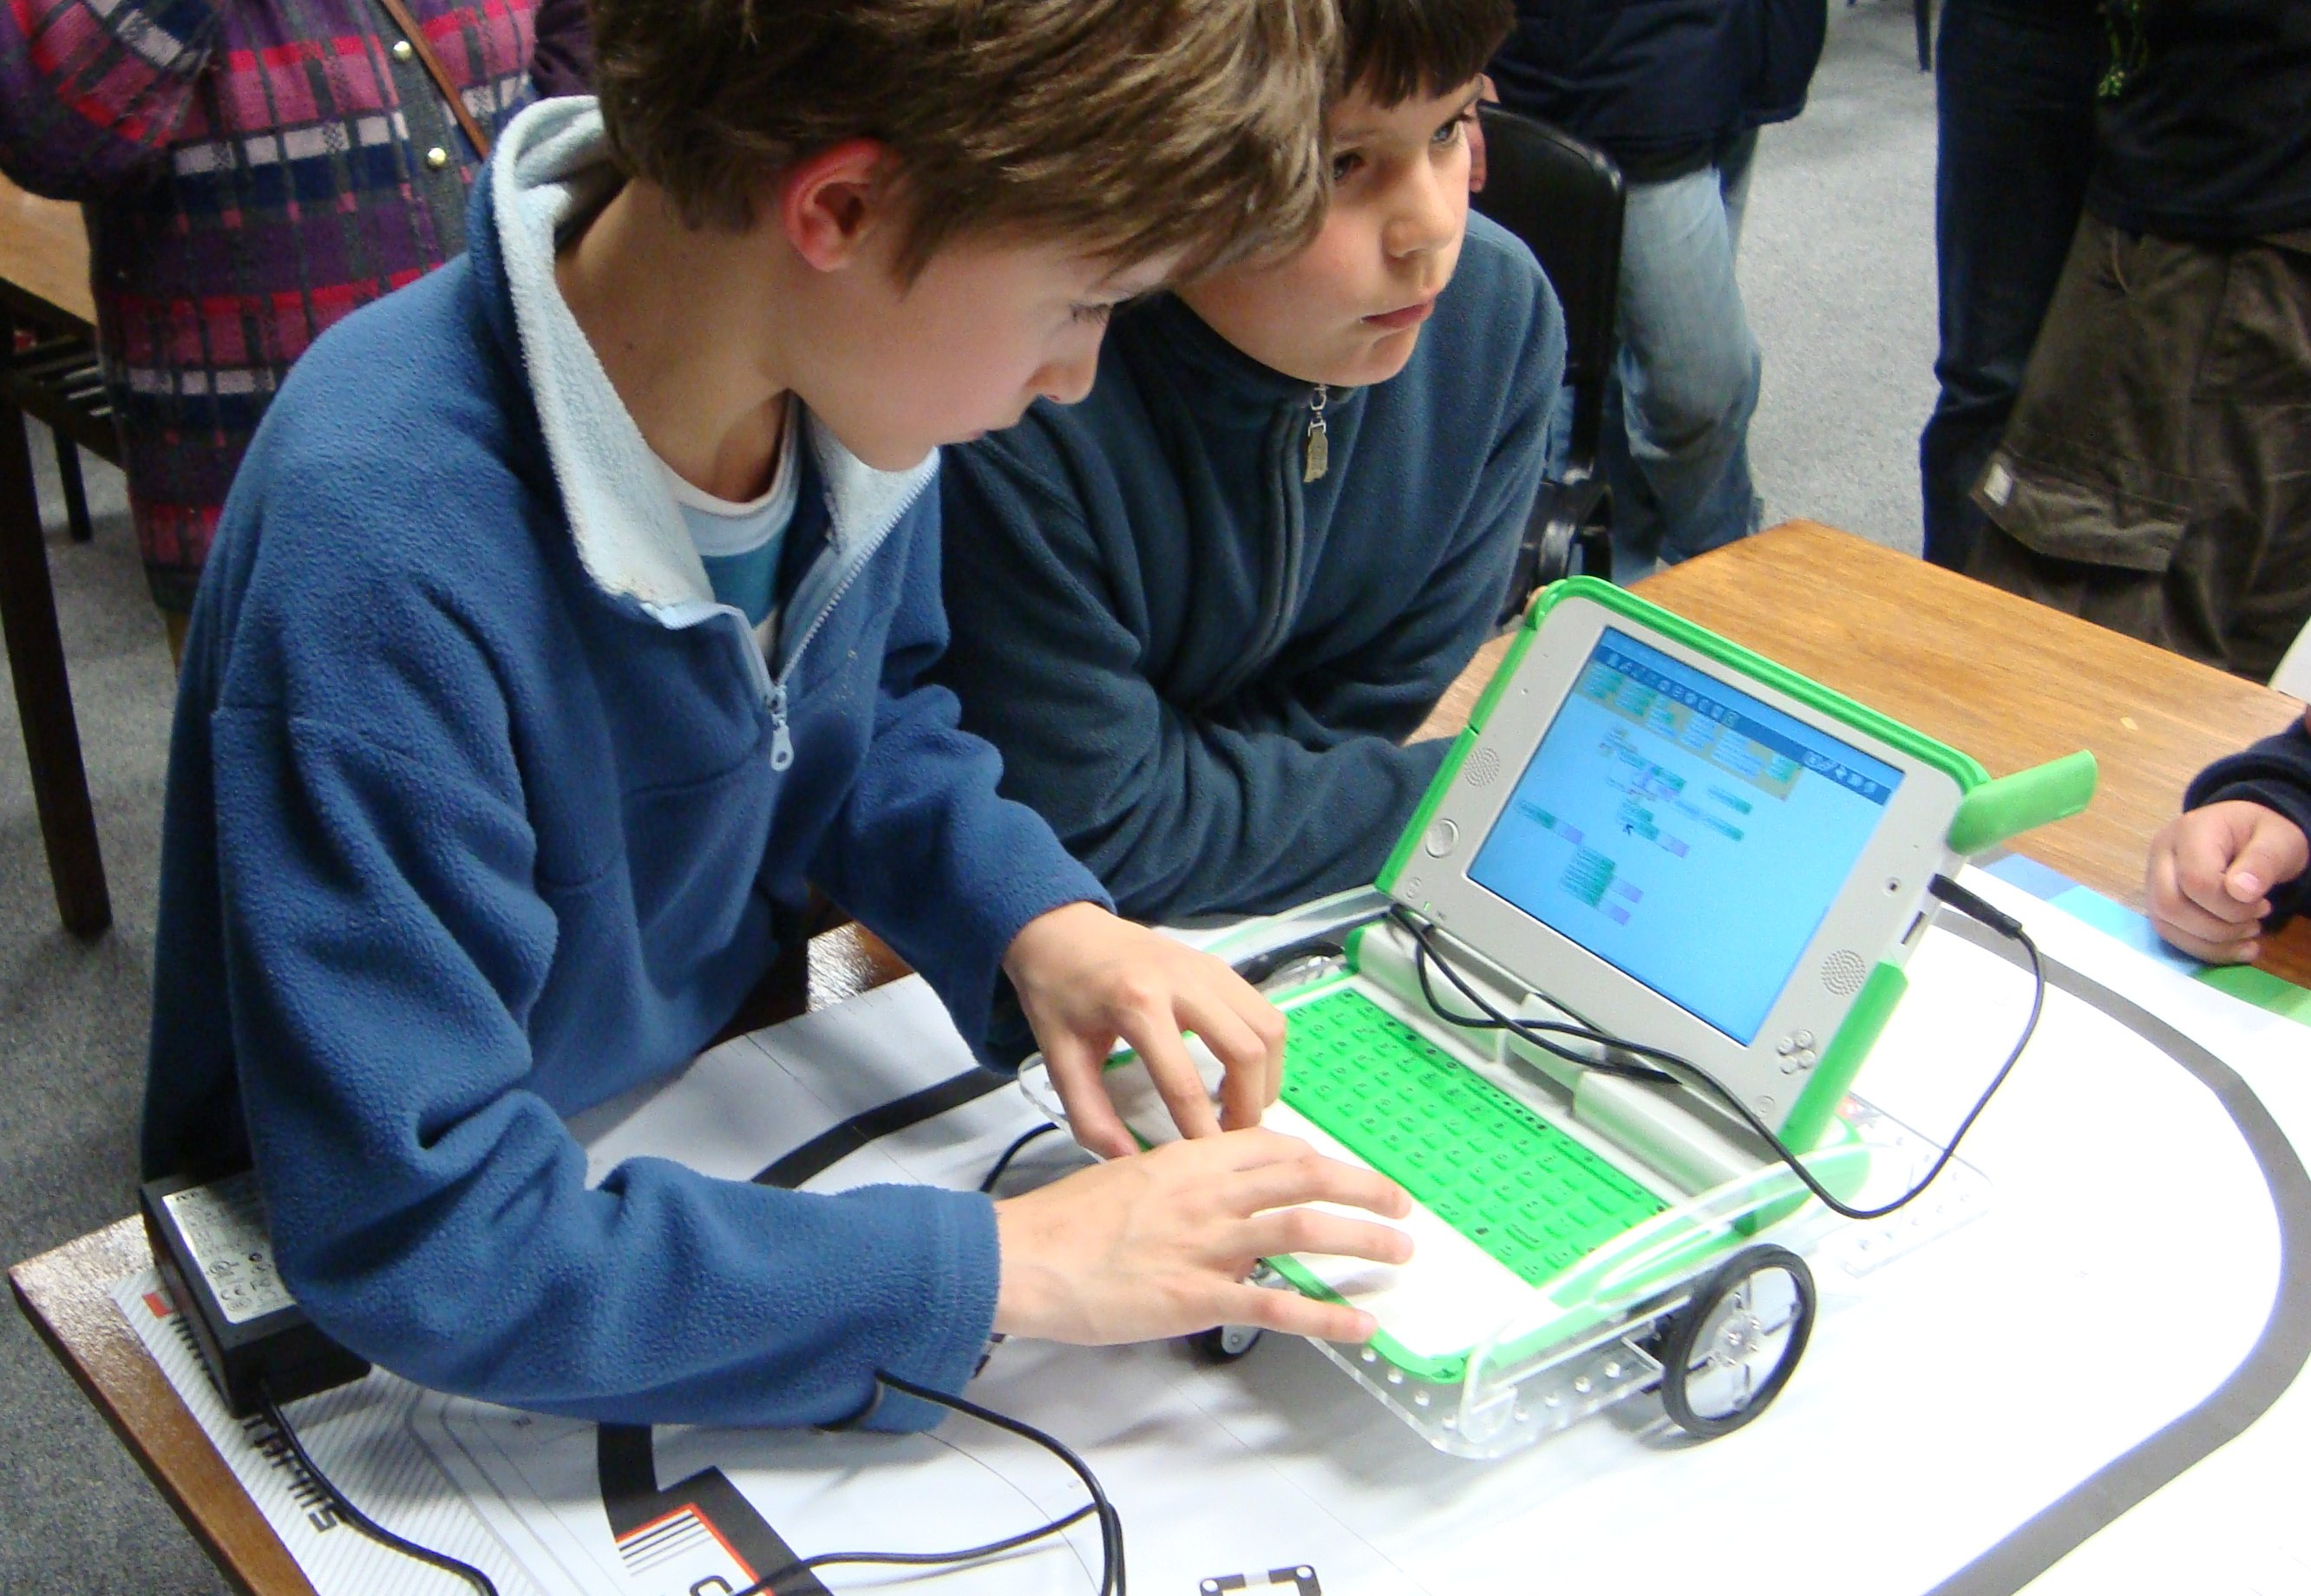
\includegraphics[scale=0.04]{graphics/pedro.JPG}
  \end{figure}
   Pedro, un usuario de tan solo 9 años
\end{center}
  \end{columns}
}


%\frame {
%  \frametitle{Programando Comportamientos}
%	   \begin{center}
%		   \begin{figure}
%		   		 Programa para evitar obstaculos desarrollado en Tortuga	
%			 	 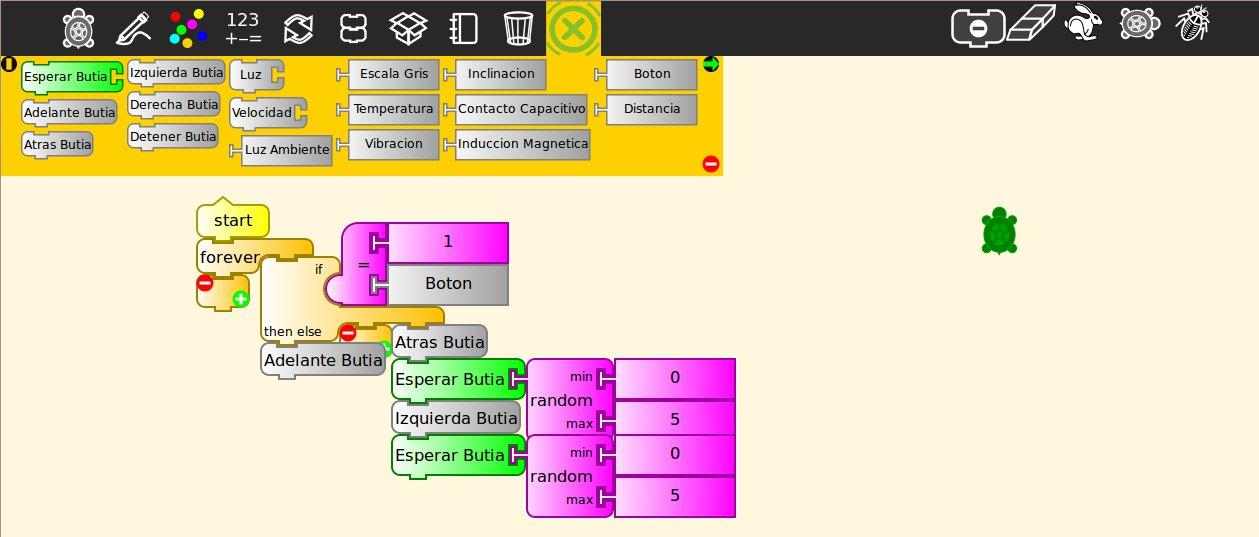
\includegraphics[scale=0.22]{graphics/tortuga_evitar_obstaculos.JPG}
%		   \end{figure}
%	   \end{center}
%}

%\frame {
%  \frametitle{Programando Comportamientos}
%	   \begin{center}
%		   \begin{figure}
%			 	 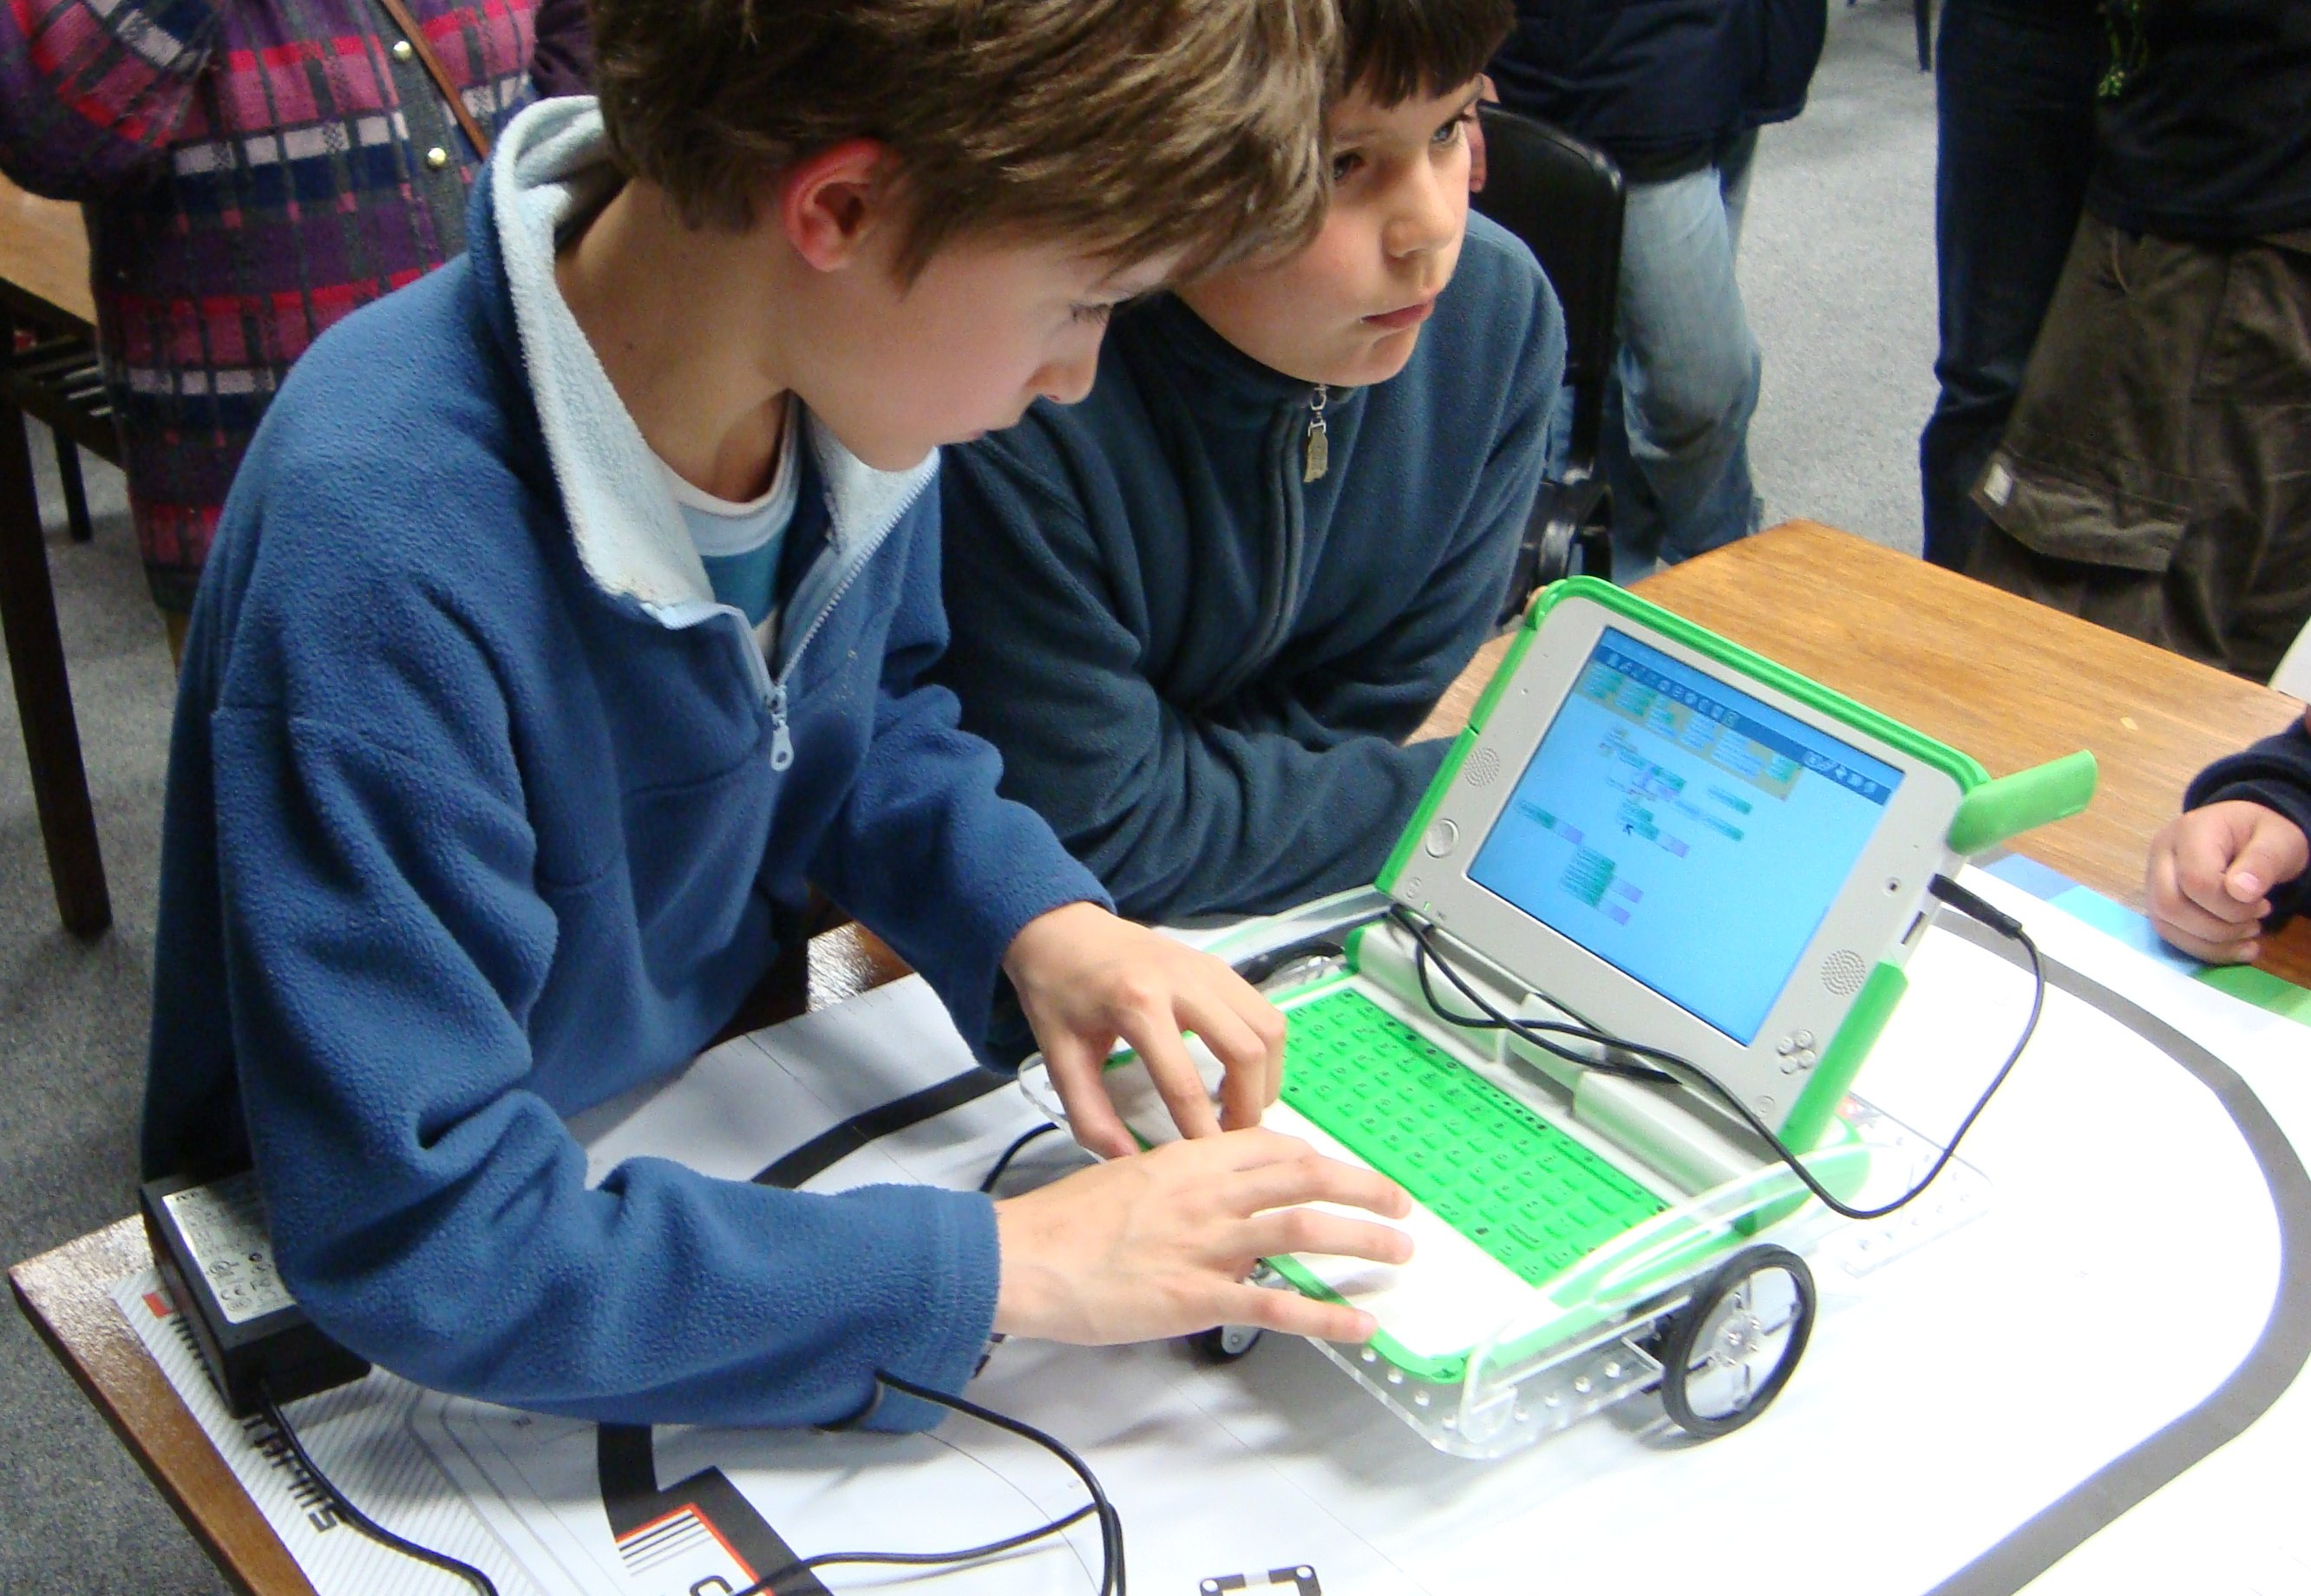
\includegraphics[scale=0.08]{graphics/pedro.JPG}
%		   \end{figure}
%	   \end{center}
%}

\subsection{Dise\~no Mec\'anico}
%FA
\frame {
  \frametitle{Chasis constructivo}
  \begin{itemize}
 	   \item Cortes en l\'aser sobre acr\'ilico
 	   \item<2-> Superficie suficiente para llevar un netbook o XO
 	   \item<3-> Orificios para colocar los sensores o actuadores
	   \item<4-> Barandas para proteger la XO
	   \item<5-> Dos ruedas de acr\'ilico las cuales est\'an sujetas a los motores
	   \item<6-> Dos ruedas locas, una de ellas amortiguada para poder sortear desniveles	
  \end{itemize}
}

\frame{
\frametitle{Hardware}
   \begin{center}
	   \begin{figure}
%			 Puertos para conectar sensores
		 	 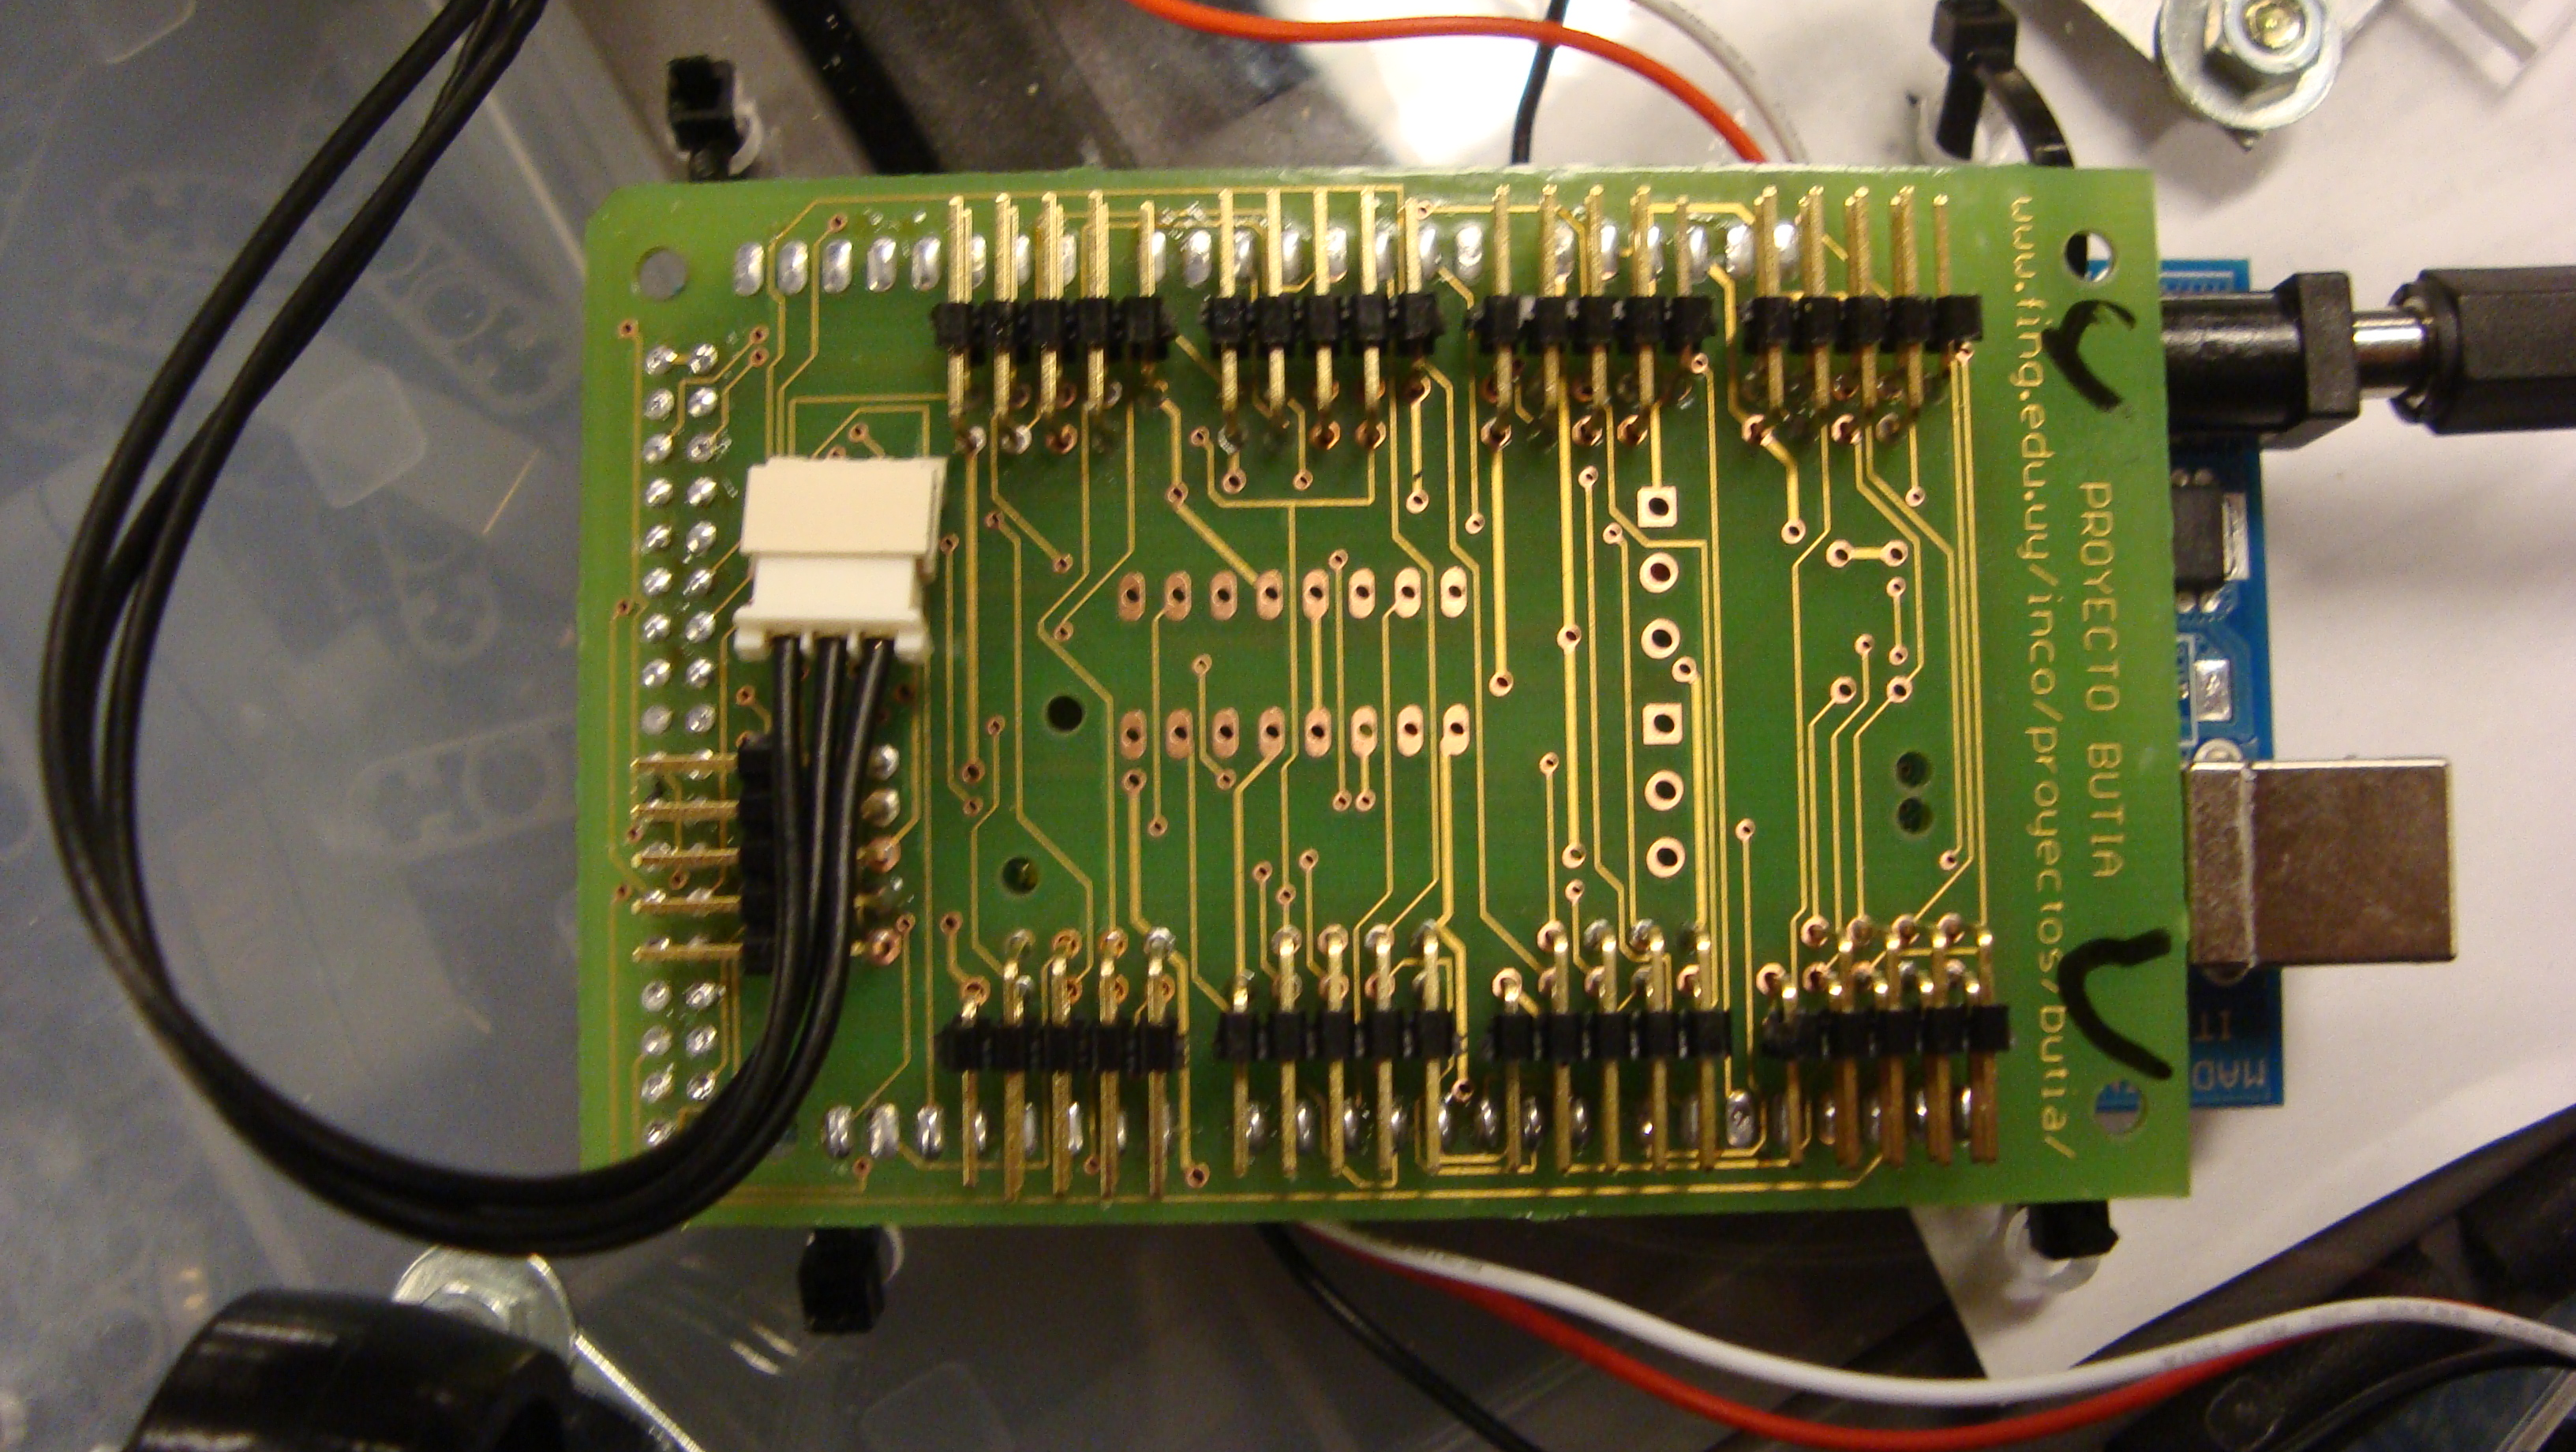
\includegraphics[scale=0.05]{graphics/shield.JPG}
	   \end{figure}
   \end{center} 
	\begin{itemize}
 	   \item Componenes de hardware:
		\begin{itemize}
	 	    \item<2-> Placa E/S basada en un microcontrolador
	 	    \item<3-> Shield dise\~nado por el grupo
			\item<4-> XO/PC/SBC
			\item<5-> Sensores/Actuadores
  		\end{itemize}  	   
  \end{itemize} 
 
}

\section{Implantaci\'on}
\subsection{Entrega de robots}
%AA
\frame {
  \frametitle{Entrega, visitas y apoyo en los liceos}
  \begin{itemize}
 	   \item<1-> El campeonato de sumo es un evento de rob\'otica realizado todos los a\~nos por la Facultad de Ingenier\'ia de la UdelaR 
		\begin{itemize}		
			\item<1-> En esta jornada se entregaron robots a 27 liceos seleccionados
			\item<1-> Se realiz\'o capacitaci\'on y talleres para estudiantes y profesores (81 personas aproximadamente)
		\end{itemize}
	   \item<2-> Durante los meses de octubre y noviembre se realizaron visitas a los liceos.
 	   \item<3-> Se realiz\'o capacitaci\'on y talleres para estudiantes y profesores (340 personas aproximadamente)
	   \item<4-> Cada liceo tiene un estudiante universitario como referente el cual le brinda apoyo y soporte.
  \end{itemize}
}

\section{Conclusiones y trabajo a futuro}
% AA
\subsection{...Buti\'a 2.0}
\frame {
\frametitle{Trabajo futuro}
 \begin{itemize}
  	\item Disminuir costos.
   	\item<2-> Portar a otros lenguajes gráficos como Scratch
 	\item<3-> Ser más eficientes con el uso de los pines para identificación
 	\item<4-> Culminar la implementación de plug \& play y shield para placa USB4all (microcontrolador PIC)
	\item<5-> Mejorar aspectos constructivos
	\item<6-> Buti\'a con elementos de desecho
	\item<7-> Incluir un brazo rob\'otico en el kit
	\end{itemize}
}

\subsection{finalmente...}
%FA
\frame {
\frametitle{Conclusiones}
 \begin{itemize}
   \item Se realizó un prototipo de robot, constructivo, totalmente integrado a la computadora utilizada por OLPC y su sistema SUGAR
   \item<2-> Se implató en 27 liceos del país
   \item<3-> Pudo validarse que incluso niños sin conocimientos previos de programación pudieron implementar fácilmente el comportamiento de robots móviles
   \item<4-> El proyecto tuvo un gran impacto en todo el país
    %estudiantes se apropiaron de la tecnología 
   \item<5-> Permitió obtener información a partir de su puesta en práctica
  \end{itemize}
}

%oculto los logos para no se solapen con las fotos
\pgfdeclareimage[height=0.0cm]{congres-logo}{graphics/SASE2011header.jpg}
\pgfdeclareimage[height=0.0cm]{butia-logo}{graphics/butia_logo.jpg}

\subsection{Más que mil palabras}
\frame{
\begin{center}
\begin{tabular}{ccc}
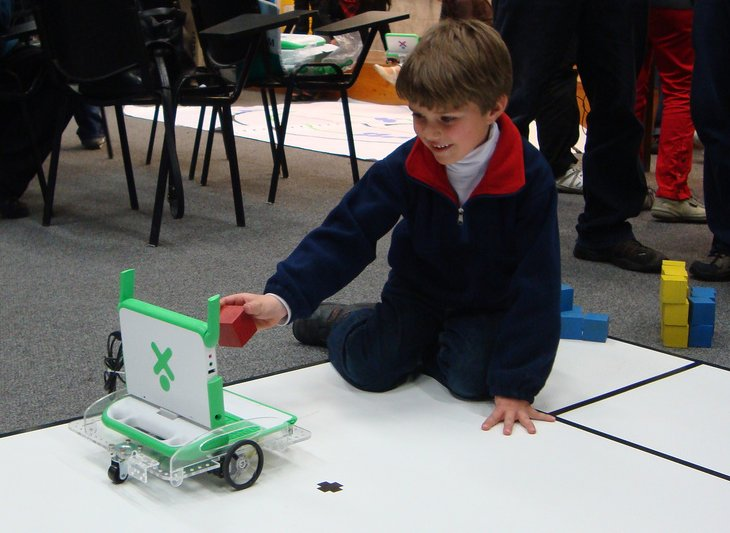
\includegraphics[width=3.8cm]{graphics/sumo-uy04} & 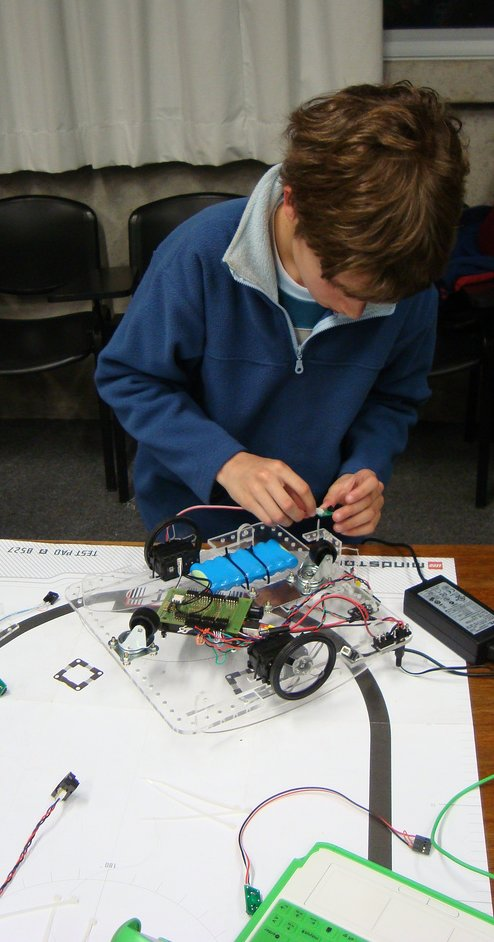
\includegraphics[width=1.45cm]{graphics/sumo-uy03} & 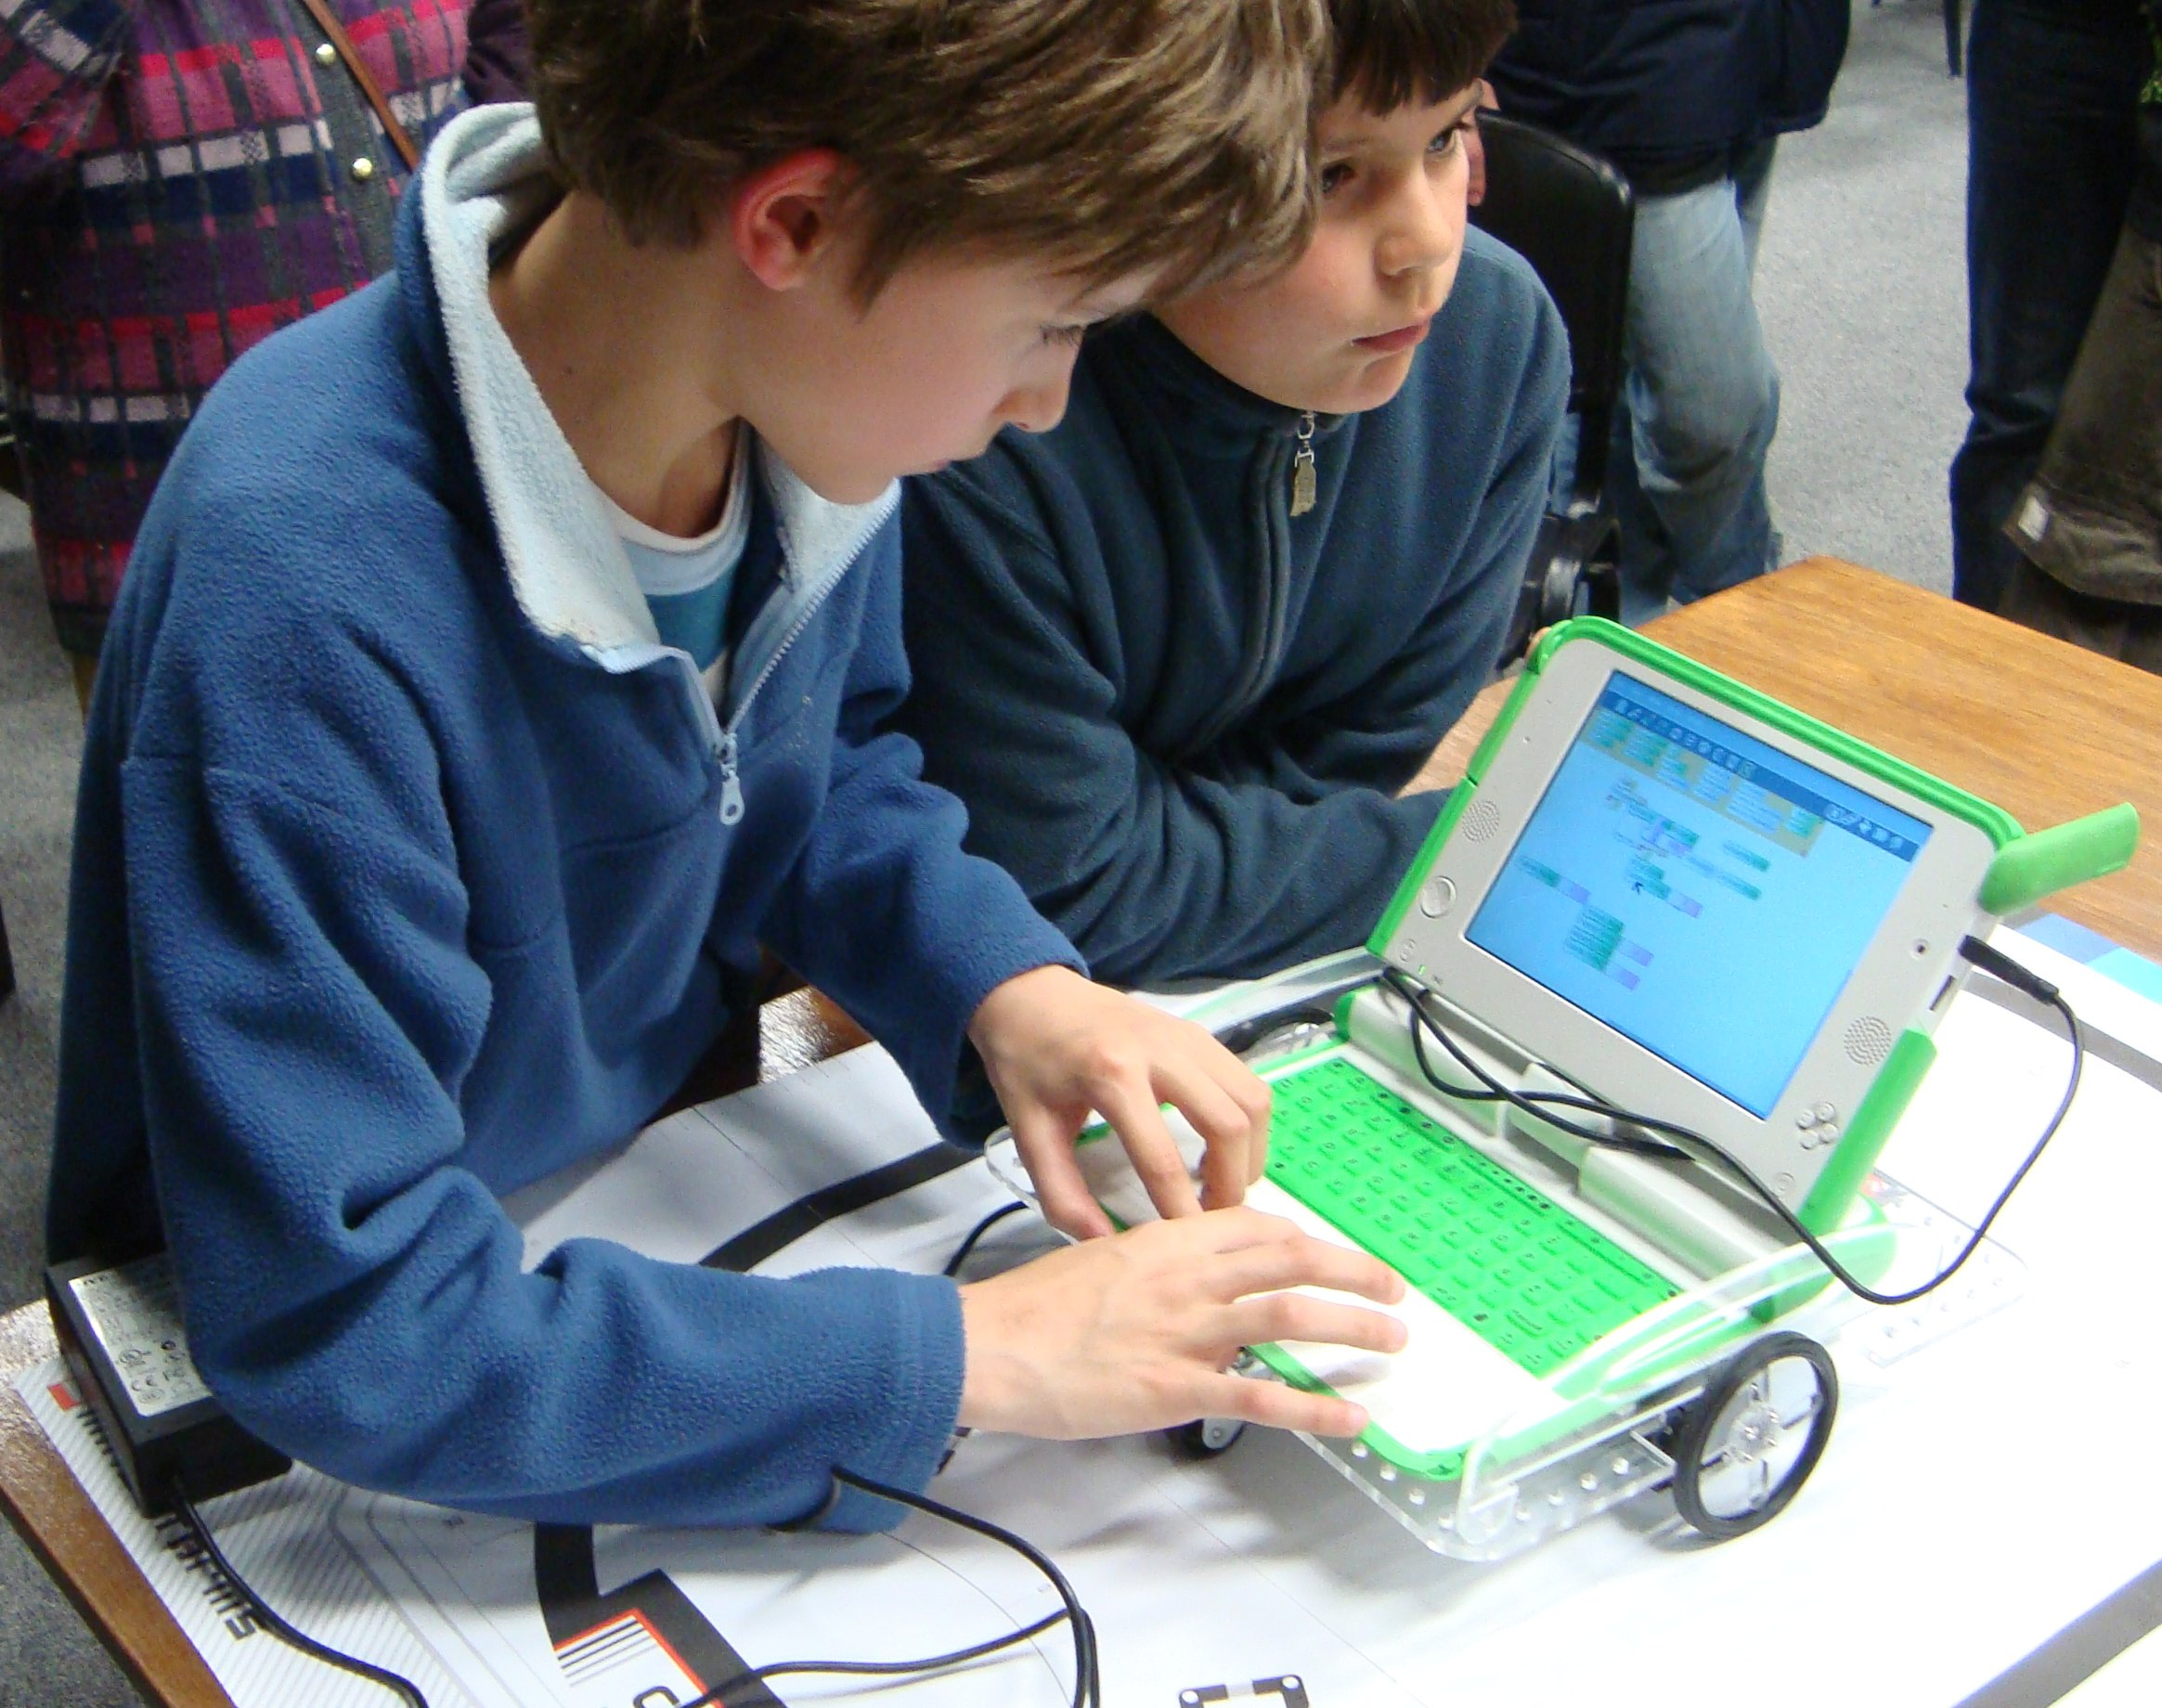
\includegraphics[width=3.55cm]{graphics/ninosProgramando}\tabularnewline
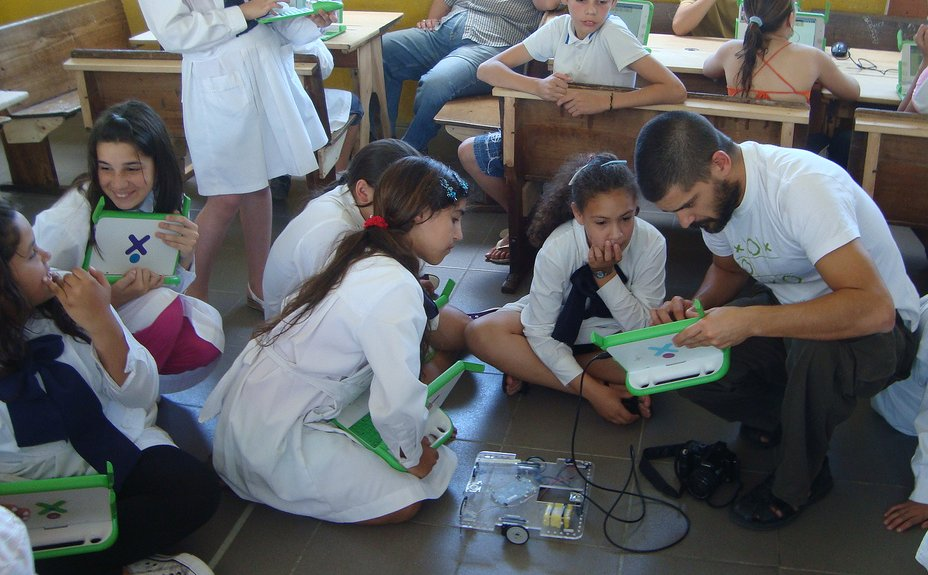
\includegraphics[width=3.8cm]{graphics/butiaEscuela} & 
\includegraphics[width=1.8cm]{graphics/logoButia} & 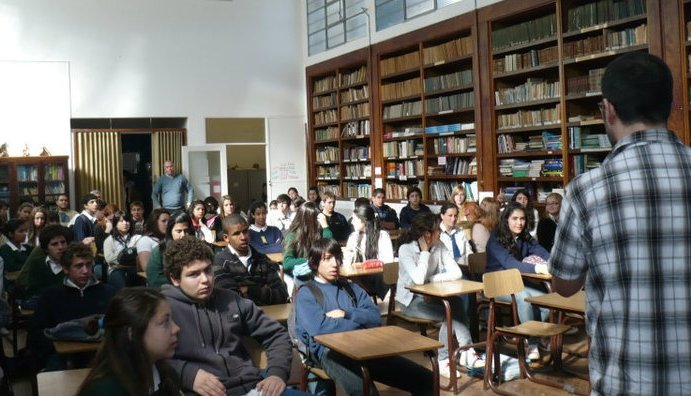
\includegraphics[width=3.8cm]{graphics/butiaLiceo02}\tabularnewline
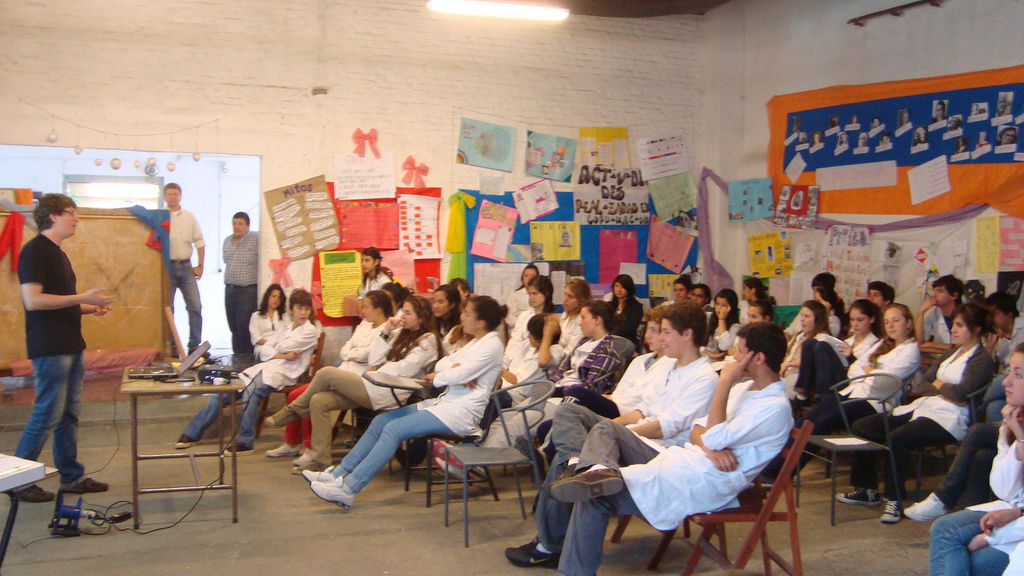
\includegraphics[width=3.8cm]{graphics/butiaLiceo01} & 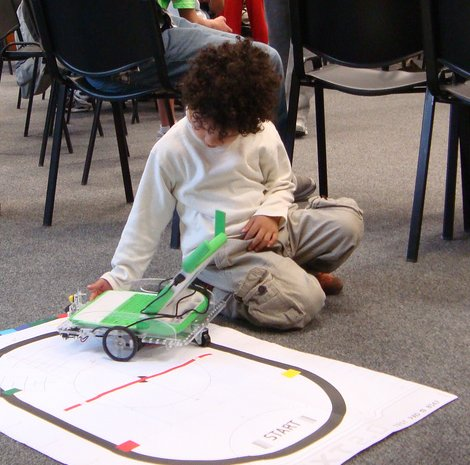
\includegraphics[width=1.9cm]{graphics/sumo-uy02} & 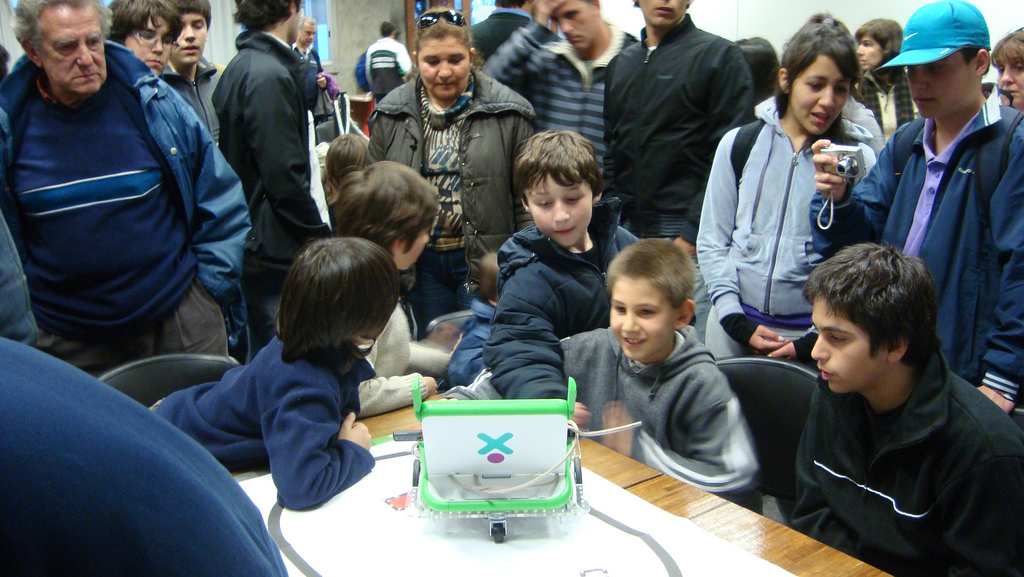
\includegraphics[width=3.8cm]{graphics/sumo-uy01}\tabularnewline
\end{tabular}
\end{center}
}

%vuelvo a colocar los logos
\pgfdeclareimage[height=0.5cm]{congres-logo}{graphics/case2011.png}
\pgfdeclareimage[height=0.5cm]{butia-logo}{graphics/butia_logo.jpg}

\subsection{Gracias por su tiempo}
\frame{
\Huge{?`Preguntas?}
\begin{center}
\begin{tabular}{cc}
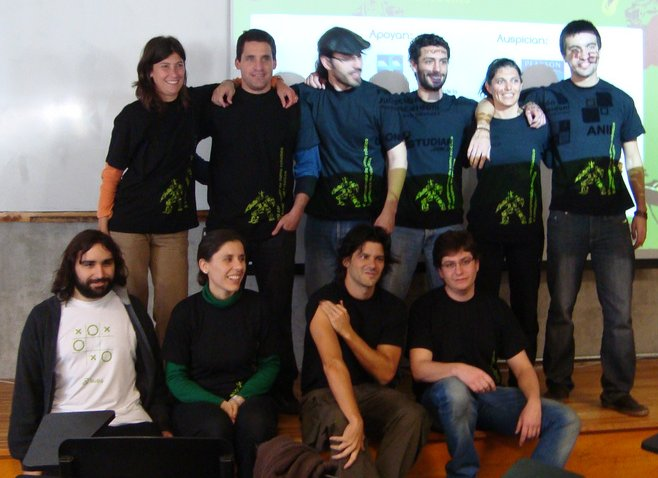
\includegraphics[width=3.8cm]{graphics/romina01} & 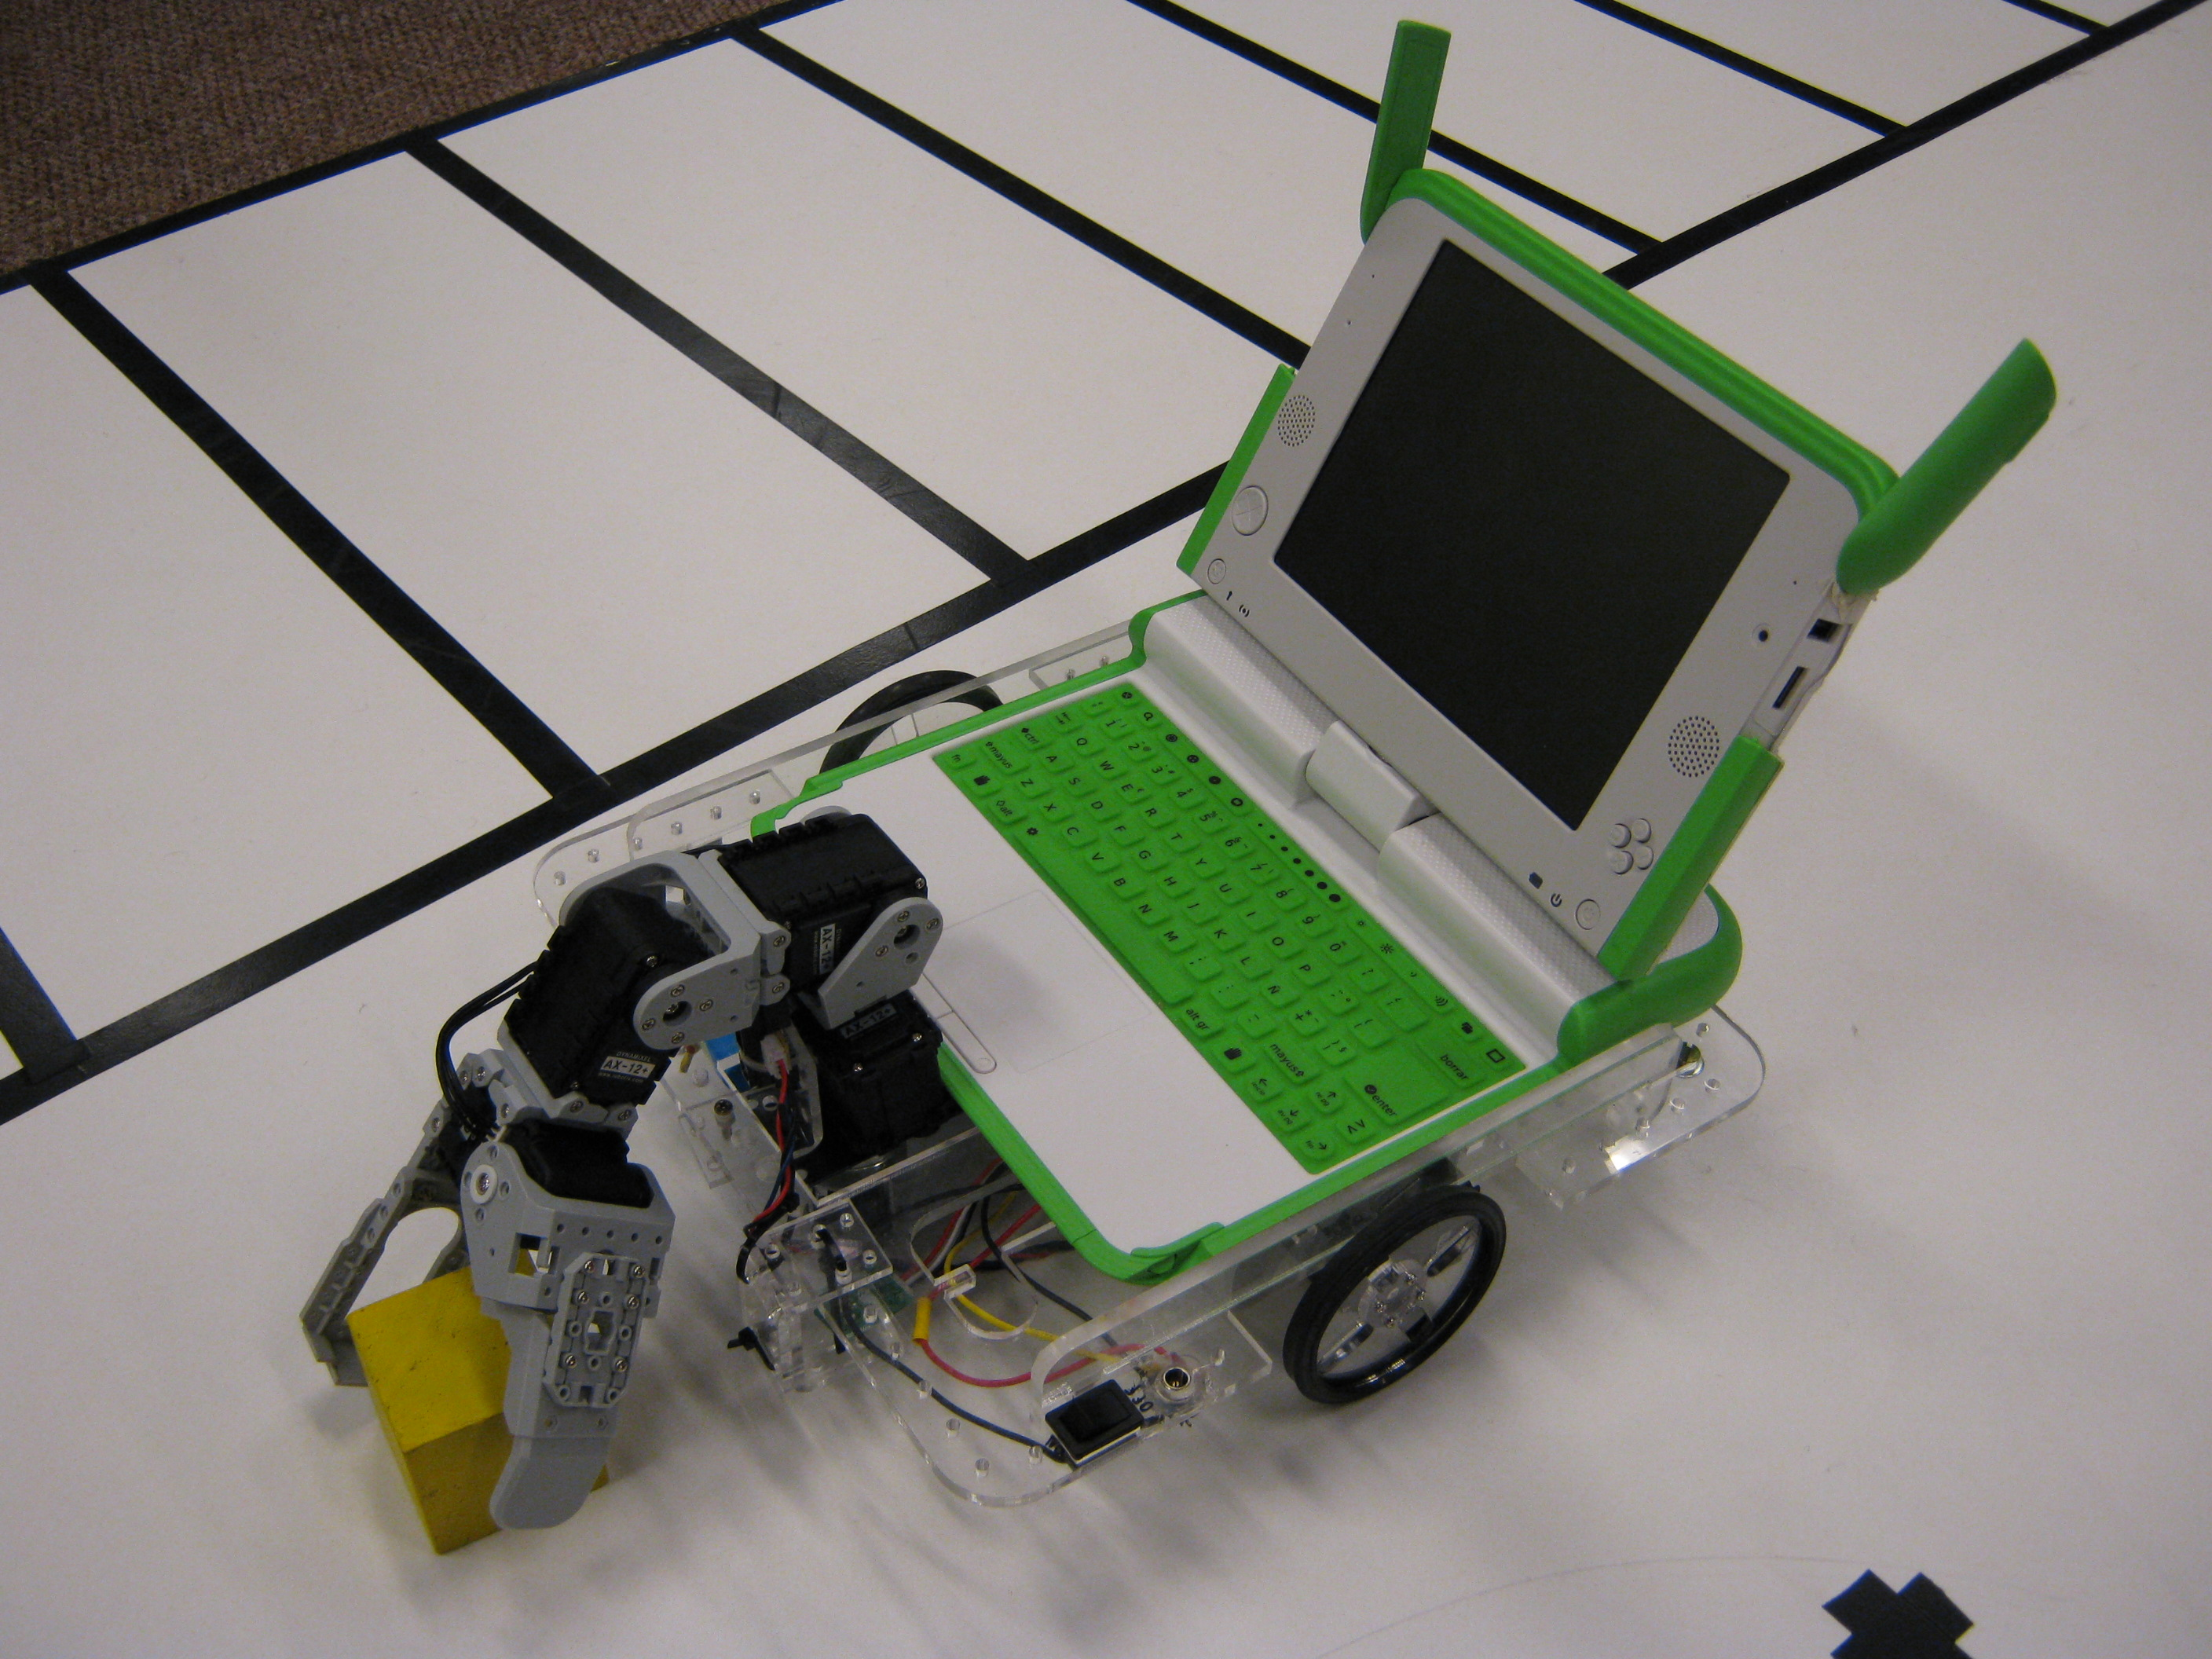
\includegraphics[width=3.8cm]{graphics/butia_pinza.JPG}\tabularnewline
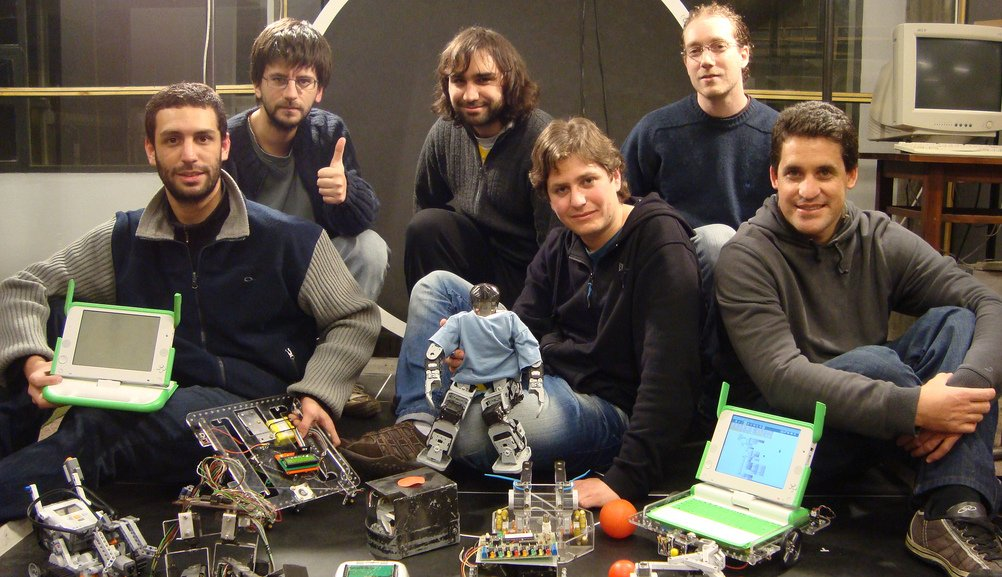
\includegraphics[width=3.8cm]{graphics/romina03} & 
\includegraphics[width=1.8cm]{graphics/logoButia} \tabularnewline
\end{tabular}
\end{center}
}

%\end{topcolumns}%{}

%\frame {
%  \frametitle{Gracias}
%\Huge{Preguntas?}
%   \begin{center}
%	   \begin{figure}
%			 Puertos para conectar sensores
%		 	 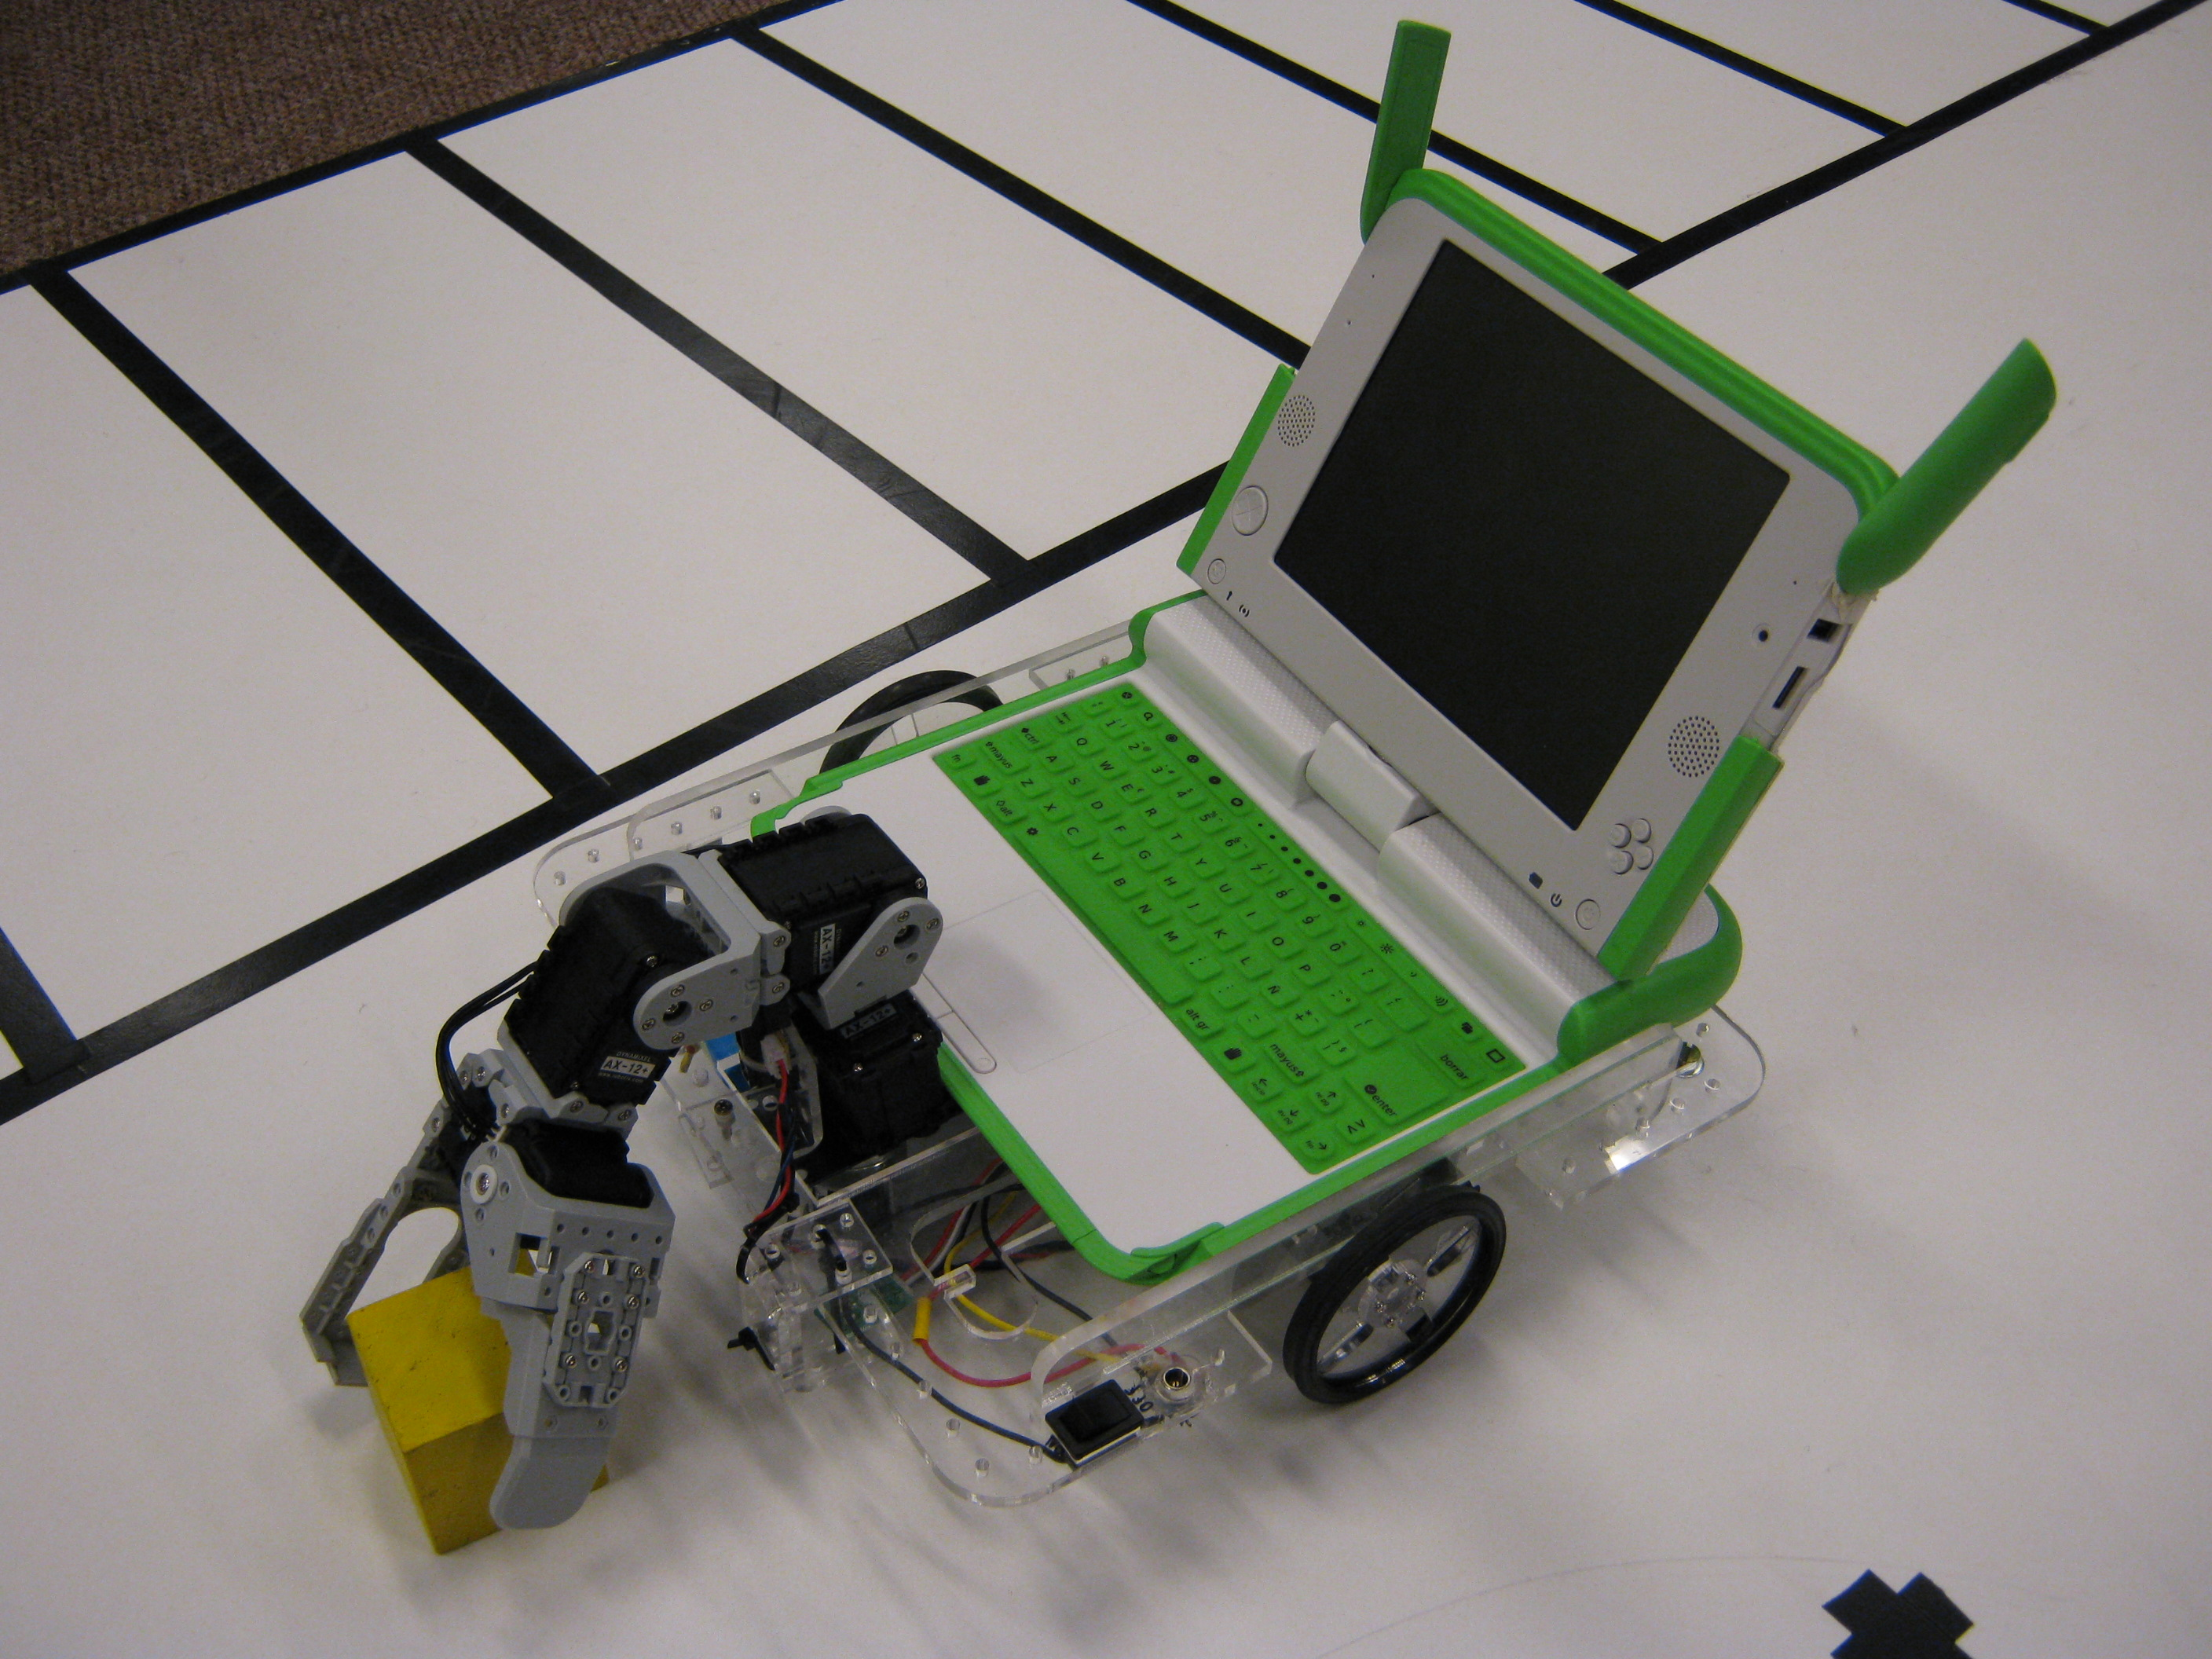
\includegraphics[scale=0.05]{graphics/butia_pinza.JPG}
%	   \end{figure}
%   \end{center}  
%}
\frame{\titlepage}

%\setbeamertemplate{background canvas}{\includegraphics[width=\paperwidth]{{graphics/bsod2.jpg}}}
%\begin{frame}[plain]
%\begin{centering}%
%\par%
%\end{centering}%
%\end{frame}

\end{document}

